\documentclass[a4paper,11pt]{article}
\usepackage[utf8]{inputenc}

% The following packages can be found on http:\\www.ctan.org
\usepackage{graphics} % for pdf, bitmapped graphics files
\usepackage{epsfig} % for postscript graphics files
\usepackage{mathptmx} % assumes new font selection scheme installed
\usepackage{times} % assumes new font selection scheme installed
\usepackage{amsmath} % assumes amsmath package installed
\usepackage{amssymb}  % assumes amsmath package installed
\usepackage{color, colortbl}
\usepackage{bm}
\usepackage{mdframed} %frame text
\usepackage{algorithmic}
\usepackage{algorithm}
\usepackage{hyperref}

%page layout: https://en.wikibooks.org/wiki/LaTeX/Page_Layout
\usepackage{fullpage}

%example counter
\newcounter{examplecounter}
%\stepcounter{examplecounter}


% define colors
\definecolor{Gray}{gray}{0.9}

%opening
\title{Some Essential Notes for Roboticists}
\author{
  Andreu Corominas-Murtra
  \thanks{
    Andreu Corominas-Murtra (andreu@beta-robots.com) is with Beta Robots (www.beta-robots.com)
    This notes are published under the Creative Commons License. In case of reference, please cite this as: Corominas-Murtra, A. Some Essential Notes for Roboticists. On-line at \url{https://github.com/andreucm/essential_maths_roboticists}. 2019. }
}

\begin{document}

\maketitle

\begin{abstract}
This document is a running collection of math notes. They try to summarize in a clear and useful way the math essentials for advanced robotics. The focus is put more on the interpretation of math entities and results, instead on computation and numerical recipes. The aim is to build a self reference tool for our daily work, and to share it. 
\end{abstract}

\newpage

\tableofcontents

\newpage
\section*{Notation}
Main conventions and notation used through the document are listed below:

$a,b,c,x,y,z,u,v,w,...$ are scalars.

$\alpha,\beta,\theta,\phi$ are also scalars, by they usually represent angles. 

$\mathbf{a,b,c,x,y,z,o,p,r,u,v,w,...}$ are vectors.

$\mathbf{M,A,B,C,F,...}$ are matrices.

$\mathbf{R}$ is a rotation matrix.

$\mathbf{T}$ is a homogeneous transform matrix.

$\mathbf{I}_n$ is the identity matrix of dimensions $n \times n$.

$\mathcal{F}^C$ is the coordinate frame (shortly, frame) of body $C$.

$\mathbf{x}^C$ is a vector referenced with respect to the $\mathcal{F}^C$ coordinate frame.

$\mathbf{a}\in \mathbb{R}^3 \rightarrow \mathbf{a} = (a_x,a_y,a_z)^T$ are the components of a vector in 3D.

$\mathbf{a}^C_x$ is the first component of $\mathbf{a}$ expressed in frame~$\mathcal{F}^C$.

$i,j,k,l,.. \in \mathbb{Z}$ are usually running index over sets. 

$t \in \mathbb{Z}$ is usually an iteration index.

$\tau \in \mathbb{R}$ is usually a timestamp.

$\tau_t \in \mathbb{R}$ is the timestamp of iteration $t$.

$m,n,p,.. \in \mathbb{Z}$ are usually vector or matrix dimensions.

$p \in \mathbb{Z}$ is also used as a degree index of some function or polynomial. 

$\mathbf{q} = (q_r,q_x,q_y,q_z) = (a,b,c,d)$ is a quaternion. $q_r$ or~$a$ are the real parts.

$\hat{\mathbf{x}}$ is an estimate of $\mathbf{x}$, which is an actual (unknown) quantity.

\newpage
\part{Math essentials}

\newpage
\input{basic_trigonometry.tex}

\newpage

\section{Basic Algebra and Calculus}

\subsection{Functions}

A real \textbf{scalar function} defined in the $\mathbb{R}^n$ domain is:
\begin{equation}
 z=f(\mathbf{x}):\mathbb{R}^n \rightarrow \mathbb{R}, 
 \ \ z \in \mathbb{R}, \ \mathbf{x} \in \mathbb{R}^n.
\end{equation}

A real \textbf{vector function} defined in the $\mathbb{R}^n$ domain is:
\begin{equation}
 \mathbf{z}=f(\mathbf{x}):\mathbb{R}^n \rightarrow \mathbb{R}^m, 
 \ \ \mathbf{z} \in \mathbb{R}^m, \ \mathbf{x} \in \mathbb{R}^n.
\end{equation}

\subsection{Norm, dot and cross products }
\label{subsec:norm_dot_cross}

The \textbf{scalar or dot product} between two vectors is:
\begin{equation}
<\mathbf{u},\mathbf{v}> = \mathbf{u}^T \cdot \mathbf{v} = \mathbf{u}^T \mathbf{v} = \sum_{i=0}^{n-1} u_{i} v_{i}
, \ \ \mathbf{u},\mathbf{v} \in \mathbb{R}^n.
\end{equation}
The scalar product is a measure of the length of the projection of one vector over the axis of the other. 
Therefore, the scalar product can be also interpreted as a measure of similarity.

The $p$-\textbf{norm} of a vector is 
\begin{equation}
 \vert \mathbf{x} \vert _p = ( \sum_{i=0}^{n-1} x_{i}^p )^{\frac{1}{p}} \ .
\end{equation}
For $p = 2$, we found the \textbf{Euclidean norm}:
\begin{equation}
 \vert \mathbf{x} \vert _2 = \vert \mathbf{x} \vert = \sqrt{\sum_{i=0}^{n-1} x_{i}^2} = \sqrt{\mathbf{x}^T \mathbf{x}}\ ,
\end{equation}
which is a measure of the length of $\mathbf{x}$, a fundamental concept.

If a vector is divided by its norm, $\frac{\mathbf{x}}{ \vert \mathbf{x} \vert }$, we obtain a \textbf{normalized} version, which can be interpreted as a vector of unit length pointing to the same direction of $\mathbf{x}$. Thus, normalized vectors indicate directions and lie on the hypersphere of unit radius. In 3D this can be interpreted as an \textbf{spherical projection}.

The scalar product between normalized $\mathbf{u}$ and $\mathbf{v}$ equals to the cosine of the angle between them:
\begin{equation}
 \frac{\mathbf{u}^T}{\vert \mathbf{u} \vert} \cdot \frac{\mathbf{v}}{\vert \mathbf{v} \vert} = 
 \frac{\mathbf{u}^T\mathbf{v}}{\vert \mathbf{u} \vert \vert \mathbf{v} \vert} =
 cos (\alpha) , \ \in [0,1]
\end{equation}
where $\alpha$ is the angle between vectors $\mathbf{u}$ and $\mathbf{v}$. This operation can be also interpreted as a similarity value between two normalized vectors. If normalized vectors are equal, the angle is 0, so the cosine is 1 (maximum similarity). Otherwise, if vectors are orthogonal, the angle is $\frac{\pi}{2}$, so the cosine results in 0 (minimum similarity). In the later case $\mathbf{u}$ and $\mathbf{v}$ span orthogonal directions. 

The \textbf{cross product} between two vectors is only defined in $\mathbb{R}^3$
\begin{equation}
 \mathbf{u} \times \mathbf{v} = \mathbf{w} , \ \ \mathbf{u},\mathbf{v},\mathbf{w} \in \mathbb{R}^3, 
\end{equation}
and results in a new vector $\mathbf{w}$ which is orthogonal to both $\mathbf{u}$ and $\mathbf{v}$. Components of the resulting vector are computed as: 
\begin{equation}
\mathbf{w} = 
\left[
\begin{array}{ccc}
  u_x\\
  u_y\\
  u_z\\
\end{array}
\right]
\times
\left[
\begin{array}{ccc}
  v_x\\
  v_y\\
  v_z\\
\end{array}
\right]
 = 
\left[
\begin{array}{ccc}
  u_y v_z - u_z v_y\\
  u_z v_x - u_x v_z\\
  u_x v_y - u_y v_x\\
\end{array}
\right]
 \end{equation}
Right hand rule, indicates forward direction of the resulting vector. That is, using the right hand, forefinger pointing as $u$, middle finger pointing following $v$, so the resulting $w$ is orthogonal to both, and points as thumb. 

\paragraph{Example \theexamplecounter. Code for norm, dot and cross products [C++/Eigen]}
\stepcounter{examplecounter}

% \begin{tcolorbox}
\begin{mdframed}
\begin{verbatim} 
#include eigen3/Eigen/Geometry 
 void main() 
 { 
    Eigen::Vector3d va; //va is a vector in R^3
    Eigen::Vector<double,3> vb; //vb is another vector in R^3
    va << 1,2,3; //fill the vector va
    vb << -1,-1,0; //fill the vector vb
    double norm_va = va.norm(); //|va|
    double dot_vab = va.dot(vb); //va^T · vb
    Eigen::Vector3d cross_vab = va.cross(vb);//va x vb 
 }  
\end{verbatim}
\end{mdframed}


\subsection{Matrix Manipulation}
A \textbf{matrix} is a rectangular array of numbers, so they are sorted in rows and columns:
\begin{equation}
\mathbf{A} \in \mathbb{R}^{m \times n}
\left[
\begin{array}{ccccc}
  a_{00} & \dots & a_{0j} & \dots & a_{0n-1} \\
  a_{10} & \dots & \dots & \dots & a_{1n-1} \\
  \dots & \dots & \dots & \dots & \dots \\
  a_{i0} & \dots & a_{ij} & \dots & a_{in-1} \\
  \dots & \dots & \dots & \dots & \dots \\
  a_{m-10} & \dots & a_{m-1j} & \dots & a_{m-1n-1} \\
\end{array}
\right]
\end{equation}
A matrix lies on a $\mathbb{R}^{m \times n}$ space, where the dimensions are the number of rows $m$, and the number of columns $n$. Element $a_{ij}$ represents a generic element of the matrix $\mathbf{A}$. Matrices are usually interpreted as a set of column or row vectors: a set of $m$ row vectors of dimension $n$, or a set of $n$ column vectors of dimension $m$. Following this interpretation, it can be written: 
\begin{equation}
\mathbf{A} = 
\left[
\begin{array}{c}
  \bar{\mathbf{a}}_0 \\
  \bar{\mathbf{a}}_1 \\
  \dots \\
  \bar{\mathbf{a}}_i \\
  \dots \\
  \bar{\mathbf{a}}_{m-1} \\
\end{array}
\right]
 = 
\left[
\begin{array}{ccccc}
  \mathbf{a}_0 & \dots & \mathbf{a}_j & \dots & \mathbf{a}_{n-1} \\
\end{array}
\right], 
\end{equation}
where $\bar{\mathbf{a}}_i$ means the row vector corresponding to row $i$. 

A matrix is called \textbf{squared} when $n=m$.

A matrix is called \textbf{diagonal} when $a_{ij}=0, \forall i\neq j$, and $a_{ij}\neq0, \forall i=j$

A matrix is called \textbf{orthogonal} when its rows or columns are orthogonal vectors, which can be checked if their scalar product is zero.  

A matrix is called \textbf{upper triangular} when $a_{ij}=0, \forall i>j$, and \textbf{lower triangular} when $a_{ij}=0, \forall i<j$.

$\mathbf{I}_n$ is the identity matrix, which is a diagonal matrix with all non-zero elements set to 1. 

The \textbf{sum} of two matrix is done element by element, so both matrix should have the same dimensions, as well as the resulting matrix:
\begin{equation}
\mathbf{A} = \mathbf{B} + \mathbf{C}, \ \mathbf{A}, \mathbf{B}, \mathbf{C} \in \mathbb{R}^{m \times n} \ \rightarrow a_{ij} = b_{ij} + c_{ij}
\end{equation}

The matrix \textbf{product}
\begin{equation}
\mathbf{A} = \mathbf{B}\ \mathbf{C}, \ 
\mathbf{A} \in \mathbb{R}^{m \times n }, 
\mathbf{B} \in \mathbb{R}^{m \times p }, 
\mathbf{C} \in \mathbb{R}^{p \times n }
\label{eq:mat_product}
\end{equation}
is computed as follows: 
\begin{equation}
a_{ij} = \bar{\mathbf{b}}_i \cdot \mathbf{c}_j = \sum_{i=0}^{p-1} b_{ip} c_{pj}. 
\end{equation}
Each resulting component can be viewed as a scalar product between $\bar{\mathbf{b}}_i$ and $\mathbf{c}_j$, 
so all comments exposed above regarding the scalar product can be interpreted for the matrix product. Please note in equation~\ref{eq:mat_product} matrix dimensions of $\mathbf{B}$ and $\mathbf{C}$, and the resulting dimensions of $\mathbf{A}$. Matrix multiplication is allowed if and only if the number of columns of the first operand is equal to the number of rows of the second operand. Therefore, matrix multiplication is not a commutative operation in a general case. 

The \textbf{rank} of a matrix is the minimum between the number of independent rows and the number of independent columns. An independent vector (row or column) means that it cannot be expressed as a linear combination of the other vectors (rows or columns) of the matrix. Therefore an independent vector adds a new dimension to the space the vectors of the matrix are spanning. 

The \textbf{matrix determinant} is defined for squared matrices, and it is computed following this recursive expression: 
\begin{equation}
det(\mathbf{A}) = |\mathbf{A}| = \sum_{j=0..n-1} (-1)^{1+j}\ a_{ij}\ det(\mathbf{A}_{-0j})
\end{equation}
where $\mathbf{A}_{-0j}$ is the matrix composed by $\mathbf{A}$ but removing its first row and column~$j$. For $n=2$ this expression is reduced to:  
\begin{equation}
\left|
\begin{array}{cc}
  a_{00} & a_{01}\\
  a_{10} & a_{11} \\
\end{array}
\right| = 
a_{00}a_{11} - a_{01}a_{10}
\end{equation}
A matrix is called rank deficient or null-rank when its determinant is zero, meaning that some row or column can be expressed as a linear combination of other rows or columns respectively.

The determinant is a measure of the hypervolume of the hyperellipsoide represented by matrix $\mathbf{A}$. 

% \paragraph{Example~\ref{par:ex_determinant}}
% \label{par:ex_determinant}
% %Deteriminant as a measure of hipervolume, eigen vectors as the direction of ellipses major and minor axis, 
% Let's see an example in 2D, where the hypervolume becomes the area. Given the matrix
% \begin{equation}
% \mathbf{A} = 
% \left|
% \begin{array}{cc}
%   1.5 & 0.5\\
%   0.5 & 2 \\
% \end{array}
% \right|
% \end{equation}
% which could be the resulting covariance matrix from some estimation process. We want to visualize what the determinant is showing, so we compute it: 
% \begin{equation}
%  |\mathbf{A}| = 1.5 \cdot 2 - 0.5 \cdot 0.5 = 2.75
% \end{equation}


The \textbf{transpose} of~$\mathbf{A}$, only defined for squared matrices, is~$\mathbf{A}^T$, where its elements exchange columns by rows: 
\begin{equation}
 \mathbf{A} = \{a_{ij}\}; \ \mathbf{A}^T =\{a_{ji}\} 
\end{equation}


Given a squared matrix~$\mathbf{A}$ of sizes $n \times n$, $\mathbf{A}^{-1}$ is the \textbf{inverse} of a $\mathbf{A}$, so it fulfills that $\mathbf{A}^{-1}$ is also squared $n \times n$ and:
\begin{equation}
 \mathbf{A}\mathbf{A}^{-1} = \mathbf{A}^{-1}\mathbf{A} = \mathbf{I}_n
\end{equation}

The following is a list of useful expressions%~\cite{henderson80}, [...]: 
\begin{align}
 (\mathbf{A}^{-1})^{-1} & = \mathbf{A} \\
 (\mathbf{A}^T)^{-1} & = (\mathbf{A}^{-1})^T \\
 (a \mathbf{A})^{-1} & = a^{-1} \mathbf{A}^{-1}\\
 (\mathbf{A}\mathbf{B})^T & = \mathbf{B}^T\mathbf{A}^T\\
 (\mathbf{A}\mathbf{B})^{-1} & = \mathbf{B}^{-1}\mathbf{A}^{-1}\\
 \mathbf{A}(\mathbf{B}+\mathbf{C}) & = \mathbf{A}\mathbf{B}+\mathbf{A}\mathbf{C}\\ 
 (\mathbf{A}+\mathbf{B})^T & = \mathbf{A}^T + \mathbf{B}^T\\
 (\mathbf{A}+\mathbf{B})^{-1} & = \mathbf{A}^{-1}-\mathbf{A}^{-1}\mathbf{B}(\mathbf{I}+\mathbf{A}^{-1}\mathbf{B})^{-1}\mathbf{A}^{-1}
\end{align} 

The following equation shows the \textbf{matrix inversion lemma}. It's a useful expression in situations where matrix $\mathbf{A}$ and~$\mathbf{C}$ are easy to invert, because they may be diagonal or have small dimension. In such case it can be applied:
\begin{equation}
 (\mathbf{A}+\mathbf{B}\mathbf{C}\mathbf{D})^{-1} = 
  \mathbf{A}^{-1}-\mathbf{A}^{-1}\mathbf{B}\mathbf{C}(\mathbf{C}+\mathbf{C}\mathbf{D}\mathbf{A}^{-1}\mathbf{B}\mathbf{C})^{-1}
  \mathbf{C}\mathbf{D}\mathbf{A}^{-1}
\end{equation}
The prove can be found at[ref], but it starts by multiplying at each side by $(\mathbf{A}+\mathbf{B}\mathbf{C}\mathbf{D})$.

The \textbf{skew-symmetric matrix} in $\mathbb{R}^3$ is defined as a square matrix whose transpose is also its negative:
\begin{equation}
\mathbf{A} = 
\left[
\begin{array}{ccc}
  0 & a & -b\\
  -a & 0 & c\\
  b & -c & 0\\
\end{array}
\right].
\end{equation}
The skew matrix can be useful to represent the vector product as a matrix-vector product. If $\mathbf{a}=[a_x,a_y,a_z]$ is a vector in $\mathbb{R}^3$, let be $\mathbf{A}$ the following matrix:
\begin{equation}
\mathbf{A}_s(\mathbf{a}) = \mathbf{A}_s 
\left[
\begin{array}{ccc}
  0 & -a_z & a_y\\
  a_z & 0 & -a_x\\
  -a_y & a_x & 0\\
\end{array}
\right], 
\end{equation}
then the vector product of $\mathbf{a}\times\mathbf{b}$ can be expressed as:
\begin{equation}
 \mathbf{a}\times\mathbf{b} = \mathbf{A}_s\mathbf{b} 
\end{equation}
A \textbf{hermitian} matrix is that fulfilling: 
\begin{itemize}
 \item $\mathbf{A}$ is square $n\times n$.
 \item $\mathbf{A} = (\mathbf{A}^T)^* \rightarrow a_{ij} = a_{ji}^*$
\end{itemize}
And a \textbf{positive-definite} matrix is that fulfilling: 
\begin{itemize}
 \item $\mathbf{A}$ is square $n\times n$.
 \item $\mathbf{v}^T\mathbf{A}\mathbf{v} > 0, \ \forall\mathbf{v}\in \mathbb{R}^n$, and $\neq \mathbf{0} $.
\end{itemize}
Both later cases are commonly found in practical robotics applications and present interesting properties exploited by algebra programming libraries.


\newpage
\input{rigid_transformations.tex}

\newpage

\section{Matrix decompositions}
Matrix decompositions are a set of methods that allow to express a single matrix as a product of several other matrix that may have special properties, such as they can be, for instance diagonal, triangular or rotation matrixes, so we can them apply properties, usually to speed up computation, or to better interpret main directions/components of a given matrix.

\subsection{Eigen Decomposition}
//TODO

\subsection{Singular Value Decomposition (SVD)}
\label{subsec:matrix_svd}

\paragraph{Definition}
Given a matrix $\mathbf{M}\in \mathbb{R}^{m\times n}$, the SVD decomposition is:
\begin{equation}
 \mathbf{M} = \mathbf{U} \mathbf{D} \mathbf{V}^T
\end{equation}
where $\mathbf{U} \in \mathbb{R}^{m\times m}$ is a squared orthogonal matrix , $\mathbf{D} \in \mathbb{R}^{m\times n}$ is a rectangular diagonal matrix with non-negative entries in the diagonal and $\mathbf{V} \in \mathbb{R}^{n\times n}$ is also a squared orthogonal matrix. Diagonal entries of $\mathbf{D}$ are known as \textbf{singular values}, while the $m$ columns of $\mathbf{U}$, as well as the $n$ columns of  $\mathbf{V}$ are called left-singular and right-singular vectors respectively. 

\paragraph{Interpretation}
In the common case of $\mathbf{M}\in \mathbb{R}^{m\times m}$, with $\vert \mathbf{M} \vert > 0$, SVD can be interpreted as a composition of three geometrical transforms: a rotation expressed by~$\mathbf{V}^T$, a scaling by~$\mathbf{D}$ and last rotation by~$\mathbf{U}$. Summarizing, $\mathbf{M}\mathbf{a}$ equals to: 
\begin{equation}
\begin{split}
 \mathbf{V}^T\mathbf{a} \rightarrow rotation\\
 \mathbf{D}(\mathbf{V}^T\mathbf{a}) \rightarrow scaling\\
 \mathbf{U}(\mathbf{D}(\mathbf{V}^T\mathbf{a})) \rightarrow rotation\\
\end{split}
\end{equation}
Singular values (entries at diagonal of $\mathbf{D}$) are the semiaxes of an ellipsoid in~$\mathbb{R}^m$. Therefore, this decomposition indicates which are the orthogonal directions spanned by a matrix. 


\paragraph{Example \theexamplecounter. SVD in 2D}
\stepcounter{examplecounter}
//TODO: Eigen and Scilab code
Given the following matrix: 
\begin{equation}
\mathbf{M} = 
\left[
 \begin{array}{cc}
  2 &  0.5 \\
  0.3 &  3 \\
 \end{array}
 \right]
\end{equation}
which is squared and with $|\mathbf{M}|>0$. Computing its SVD with a computer library leads to the following result: 
\begin{equation}
\small
\mathbf{U} = 
\left[
 \begin{array}{cc}
    0.349802   &  0.936824  \\
    0.936824  & - 0.349802 \\
 \end{array}
 \right];\ \ 
\mathbf{D} = 
\left[
 \begin{array}{cc}
    3.142312   &  0.         \\
    0.          &  1.861687  \\
 \end{array}
 \right];\ \ 
\mathbf{V} = 
\left[
 \begin{array}{cc}
    0.312080 &    0.950056  \\
    0.950056 &  - 0.312080  \\
 \end{array}
 \right];\ \ 
\end{equation}
We can check that $\mathbf{M} = \mathbf{U} \mathbf{D} \mathbf{V}^T$

\paragraph{Relation with Eigen Decomposition}
The following relations hold between Eigen values and Singular values:
\begin{itemize}
 \item The left-singular vectors of~$\mathbf{M}$ are Eigenvectors of~$\mathbf{M}\mathbf{M}^T$. 
 \item The right-singular vectors of~$\mathbf{M}$ are Eigenvectors of~$\mathbf{M}^T\mathbf{M}$.
 \item The non-zero singular values of $\mathbf{M}$ (diagonal entries of~$\mathbf{D}$), are the square root of the non-zero Eigenvalues of both~$\mathbf{M}\mathbf{M}^T$ and~$\mathbf{M}^T\mathbf{M}$. 
\end{itemize}


\subsection{Cholesky}
\paragraph{Definition}
Cholesky decomposition allows to express a hermitian and positive-definite matrix~$\mathbf{A}$ as:
\begin{equation}
 \mathbf{A} = \mathbf{L}\mathbf{L}^*
\end{equation}
where $\mathbf{L}$ is a lower triangular matrix, with entries $l_{ij}\in \mathbb{R}^+$. Matrix~$\mathbf{A}$ has a unique Cholesky decomposition.

\paragraph{Use in System Solving}
Given a linear system with vector $\mathbf{x}$ as the unknown:
\begin{equation}
 \mathbf{A}\mathbf{x} = \mathbf{b}
\end{equation}
It can be solved by executing the following steps: 
\begin{itemize}
 \item $\mathbf{L} \leftarrow Cholesky(\mathbf{A})$
 \item Solve $\mathbf{L}\mathbf{y}=\mathbf{b}$ by forward substitution.
 \item Solve $\mathbf{L}^*\mathbf{x}=\mathbf{y}$ by backward substitution.
\end{itemize}


\subsection{QR}
//TODO


\newpage
\input{differentation.tex}

%\newpage
%\input{linearization.tex}

\newpage
\section{Random Variables}
\label{sec:random_variables}
A \textbf{random variable}, $\tilde{x}$, is a mathematical representation of a value and its associated uncertainty. Usually, we are interested not just in the behaviour of a certain value of a variable or parameter, but also in how it behaves when it is uncertain. A \textit{sample} of such random variable can take several values according some \textbf{distribution law}. So we are specially interested in how this distribution law \textit{reshapes} when passing through different physical processes and/or computation steps. The \textbf{probability density function}, also known as PDF, or just \textit{density}, is a function 
\begin{equation}
F_{\tilde{x}}(x):\mathbb{R}\rightarrow \mathbb{R} 
\end{equation}
that expresses which values in the domain of the variable $x$ are more likely, according to the random variable $\tilde{x}$. However, since this function is a density, the actual value expressing a probability is the integral between an interval:
\begin{equation}
p(a<\tilde{x}<b) = \int^b_a F_{\tilde{x}}(x) dx 
\end{equation}

A \textbf{random vector}, $\tilde{\mathbf{x}}$, is an array of random variables, stacked forming a column vector: 
\begin{equation}
\tilde{\mathbf{x}} =
\left[
\begin{array}{c}
 \tilde{x}_1\\
 \tilde{x}_2\\
 \vdots \\
 \tilde{x}_n\\
\end{array}
\right].
\end{equation}
In such case, the probability density function is defined as: 
\begin{equation}
F_{\tilde{\mathbf{x}}}(\mathbf{x}):\mathbb{R}^n\rightarrow \mathbb{R} 
\end{equation}
and the probability in a given interval,~$I$, is computed as:
\begin{equation}
p(\tilde{\mathbf{x}}\in I) = 
p(a_n<\tilde{x}_1<b_n,\dots,a_n<\tilde{x}_n<b_n) = 
\int^{b_1}_{a_1} \dots \int^{b_n}_{a_n} F_{\tilde{\mathbf{x}}}(\mathbf{x}) dx_n \dots dx_1 
\end{equation}

\subsection{Moments}
A way to parameterize a distribution law is through its \textit{moments}, a set of parameters that can fully describe the distribution in some cases, or just approximate it in others. The most known moments are the mean, $\mu$, which is the fisrt order moment, and the variance, $\sigma^2$, which is the second order moment.

In the unidimensional case, from a set of $p$ samples $\{x_1\dots x_p\}$, $x_i \in\mathbb{R}$, the mean and variance can be estimated as:
\begin{equation}
 \mu_x = \frac{1}{p}\sum^p_{k=1} x_k;\ \ \ \sigma^2_x = \frac{1}{p-1}\sum^p_{k=1} (x_k-\mu_x)^2;
\end{equation}

In the multivariate case the mean becomes a vector, $\boldsymbol\mu_x\in\mathbb{R}^n$. Given~$p$ samples, it can be estimated as:
\begin{equation}
 \boldsymbol\mu_x = \frac{1}{p}\sum^p_{k=1} \mathbf{x}_k;
\end{equation}
In that multivariate case, the second order moment can be \textit{cross}computed, so a \textit{covariance} matrix is used to describe the second order stathistics, which has the following squared form: 
\begin{equation}
 \mathbf{C}_x = 
 \left[
 \begin{array}{cccccc}
  c_{11} & \dots & \dots & c_{1j} & \dots & c_{1n} \\
  \vdots &       &       & \vdots &       & \vdots \\
  c_{i1} & \dots & \dots & c_{ij} & \dots & c_{in} \\
  \vdots &       &       & \vdots &       & \vdots \\
  c_{n1} & \dots & \dots & c_{nj} & \dots & c_{nn} \\
 \end{array}
 \right];
\end{equation}
From a set of~$p$ samples, the element $c_{ij}$ of the covariance matrix is estimated as follows: 
\begin{equation}
 c_{ij} = \frac{1}{p-1}\ (\mathbf{s}_{x_i}-\mu_{x_i})^T \cdot (\mathbf{s}_{x_j}-\mu_{x_j})
\end{equation}
where $\mathbf{s}_{x_i}$ is a vector stacking all $p$ samples of component~$i$ of the random variable~$\tilde{\mathbf{x}}$, and a subtracting a scalar from a vector means that we substract the scalar at all components of the vector. 

\paragraph{Interpretation of Covariance Matrix}
Recalling the interpretation of the scalar product as a measure of similarity between two vectors (subsection~\ref{subsec:norm_dot_cross}), the element $c_{ij}$ of a covariance matrix is encoding the alignment between the components~$i$ and~$j$ of the random variable~$\tilde{\mathbf{x}}$ in the set of~$p$ samples, once the mean is subtracted. Two components that suffer from the similar variations in the sample set, will appear as two vectors~$\mathbf{s}_{x_i}$ and~$\mathbf{s}_{x_j}$ nearly aligned, so its covariance~$c_{ij}$ will be close to $\frac{1}{p-1}$. In contrast, two components of the random variable~$\tilde{\mathbf{x}}$ that change without any relation, lead to two vectors~$\mathbf{s}_{x_i}$ and~$\mathbf{s}_{x_j}$ unaligned, so the scalar product, and thus the $c_{ij}$, will approach to~$0$.

So, the covariance matrix builds a base of $n$ vectors (not necessarily orthogonal!) in the space of the random variable~$\tilde{\mathbf{x}}$ with directions according how individual components behave similarly or not in the dataset of~$p$ samples. SVD decomposition can be applied to find out the main orthogonal directions of this base. 

\paragraph{Example \theexamplecounter. Compute a 2D covariance matrix from data [Scilab].}
\stepcounter{examplecounter}
In this example we'll generate two sample sets $S_1$ and $S_2$, each one composed by $100$ samples in~$\mathbb{R}^2$, so $100$ points $(x,y)$. $S_1$~is built forcing a strong linear relation between first and second component, while~$S_2$ is just computed by drawing random values for both components. The code below computes the covariance matrix for both sets.
\begin{mdframed}
\tiny
\begin{verbatim} 
//user entries
mm = 0.3;
bb = 0;
noise_stdev = 0.3; //sqrt(noise_variance)

//create set S1
xx1 = [0:0.1:10]';
[nn cols] = size(xx1); //get set size
yy1 = mm*xx1 + bb + noise_stdev*rand(nn,1,"normal");

//create set S2
xx2 = noise_stdev*rand(nn,1,"normal");
yy2 = noise_stdev*rand(nn,1,"normal");

//compute means, each component, each set:
mx1 = sum(xx1)/nn;
my1 = sum(yy1)/nn;
mx2 = sum(xx2)/nn;
my2 = sum(yy2)/nn;

//compute covariance matrix explicitly
cxx1 = (xx1-mx1)'*(xx1-mx1)/(nn-1);
cyy1 = (yy1-my1)'*(yy1-my1)/(nn-1);
cxy1 = (xx1-mx1)'*(yy1-my1)/(nn-1);
cxx2 = (xx2-mx2)'*(xx2-mx2)/(nn-1);
cyy2 = (yy2-my2)'*(yy2-my2)/(nn-1);
cxy2 = (xx2-mx2)'*(yy2-my2)/(nn-1);

//compute covariance matrix with scilab call
C1 = cov(xx1,yy1);
C2 = cov(xx2,yy2);
\end{verbatim} 
\end{mdframed}
The resulting covariance matrices are:
\begin{equation}
\small
\mathbf{C}_1 = 
\left[
 \begin{array}{cc}
    8.585      &  2.6312156  \\
    2.6312156  &  0.8963398  \\
 \end{array}
 \right];\ \ 
\mathbf{C}_2 = 
\left[
 \begin{array}{cc}
    0.0930911  & - 0.0006647  \\
  - 0.0006647  &  0.0884355   \\
 \end{array}
 \right];\ \ 
\end{equation}
The resulting matrices show how the set $S_1$ presents a much higher relation between~$x$ and~$y$ components than~$S_2$, due to the linear relation imposed when building the sets. Moreover, the fact that the values in~$C_1$ are much larger is caused because~$S_1$ stretches in the $XY$ plane occupying a larger region than~$S_2$.

\paragraph{Example \theexamplecounter. Ellipses from a 2D covariance matrix.}
\stepcounter{examplecounter}
This example shows a Scilab function to draw a 2D ellipses from a covariance matrix, centered at a given $(x,y)$ point. Numerical errors can lead to non-positive-definite covariance matrixes after some computational steps. Therefore, the first calls in the function are related to ensure that the matrix is strictly positive-definite, a necessary condition to assure eigenvalues are real (TBC!!). Positive-definite is ensured through a Cholesky decomposition. Thereafter, eigenvalues are computed, which directly provide the length of a major and minor axes of the ellipses. Finally, drawing is performed point by point over the ellipses, with steps of $0.1$ radian. 
\begin{mdframed}
\tiny
\begin{verbatim} 
//covariance matrix Cmat, and centered at point mu
function[] = draw_ellispes_from_cov(mu, Cmat, axes_h)

    //ensure positive-definite matrix
    Cchol = chol(Cmat);
    CC = Cchol'*Cchol;  
    
    //compute eigenvalues
    [RR,diagCC] = spec(CC);
    eval1 = diagCC(1,1);
    eval2 = diagCC(2,2);
    
    //sort evals by value. Set major and minor axes.
    if (eval1>eval2) then
        axis = [eval1;eval2;atan(RR(2,1)];
    else
        axis = [eval2;eval1;atan(RR(2,2)];
    end

    //start drawing (compute all points) 
    step = 0.1; //Set drawing step    
    t = 0:step:%pi/2; //set drawing vector
    eX = axis(1)*cos(t); //ellispes points (X component, a quarter)
    eY = axis(2)*sin(t); //ellipses points (Y component, a quarter)
    nn = 4*size(eX,'*'); //num of total points of the ellipses
    eXY1 = [eX, -flipdim(eX,2), -eX, flipdim(eX,2); eY, flipdim(eY,2), -eY, -flipdim(eY,2)];
    eXY = rotate(eXY1, axis(3)) + [mu(1)*ones(1,nn);mu(2)*ones(1,nn)];
    sca(axes_h); //Set current axes
    xpoly(eXY(1,:), eXY(2,:));

endfunction
\end{verbatim} 
\end{mdframed}




% \paragraph{Example \theexamplecounter. Bounding box from a set of 2D points.}
% \stepcounter{examplecounter}


% \subsection{Higher order moments}
% Third and fourth order moments are called skewness and kurtosis.  

\subsection{Uniform distribution}
A random variable or vector is called uniform when the density is constant over a bounded interval, meaning that the variable is equally distributed within this interval. That implies also that the variable can take, with equal probability, values within this interval. 

Uniform random variables can be described with just two parameters: $x_{min}, x_{max}$. The mean and the variance values of an unfiorm random variable are:
\begin{equation}
 \mu_{\tilde{x}} = \frac{x_{min}+x_{max}}{2}; \ \ \sigma^2_{\tilde{x}} = \frac{1}{12}(x_{max}-x_{min})^2
\end{equation}
%TODO: Example of C++/std code for uniform random generator}

\subsection{Gaussian distribution}
A random variable is called Gaussian or Normal, when its density is fully described with two parameters, $\mu_{\tilde{x}}$ (mean) and $\sigma^2_{\tilde{x}}$ (standard deviation), and the following expression:
\begin{equation}
 F_{\tilde{x}}(x) = \frac{1}{2\pi}e^{-(\frac{x-\mu_{\tilde{x}}}{\sigma_{\tilde{x}}})^2}
\end{equation}
Gaussian variables are also written as $\mathcal{N}(\mu,\sigma)$, which is a widely used notation stressing the dependency with just two parameters. Given $\tilde{x}=\mathcal{N}(\mu_x,\sigma_x)$ and $\tilde{y}=\mathcal{N}(\mu_y,\sigma_y)$, the following properties fulfill:
\begin{itemize}
 \item $\tilde{z}=a\tilde{x} \ \rightarrow \tilde{z}=\mathcal{N}(a\mu_x,a\sigma_x)$
 \item $\tilde{z}=\tilde{x}+\tilde{y} \ \rightarrow \tilde{z}=\mathcal{N}(\mu_x+\mu_y,\sqrt{\sigma^2_x+\sigma^2_y})$
\end{itemize}
The two properties listed above are of major importance since they imply that we know how Gaussian variables behave when they pass through linear systems. 
%example code for normal random generator and then computation of mean and variance

\subsection{Multivariate Gaussian distribution}
\label{subsec:mulivariate_gaussian_distribution}
In case of $n$-dimensional Gaussian variables, the mean is $\boldsymbol{\mu} \in \mathbb{R}^n$, and the covariance is represented as a squared matrix, $\mathbf{C}\in\mathbb{R}^{n\times n}$. The generalized formula is the following: 
\begin{equation}
 F_{\tilde{x}}(\mathbf{x}) = \frac{1}{\sqrt{\vert \mathbf{C}\vert}(2\pi)^n}
			    e^{-\frac{1}{2}(\mathbf{x}-\boldsymbol\mu)^T\mathbf{C}^{-1}(\mathbf{x}-\boldsymbol\mu)}
\end{equation}
\begin{figure}[bth!]
  \begin{center}
    \includegraphics[width=1.0\columnwidth]{figures/mv_gaussian.eps}
    \caption{Bivariate Gaussian function}
    \label{fig:mv_gaussian}
  \end{center}
\end{figure}

In the multivariate case, the properties around the sum and the linear operation also fulfill: 
\begin{itemize}
 \item $\tilde{\mathbf{z}}=\mathbf{A}\tilde{\mathbf{x}} \ 
      \rightarrow \tilde{\mathbf{z}}=\mathcal{N}(\mathbf{A}\boldsymbol\mu_x,\mathbf{A}\mathbf{C}_x\mathbf{A}^T)$, 
      where $\mathbf{A}\in \mathbb{R}^{m \times n}$.
 \item $\tilde{\mathbf{z}}=\tilde{\mathbf{x}}+\tilde{\mathbf{y}} \ 
      \rightarrow \tilde{\mathbf{z}}=\mathcal{N}(\boldsymbol\mu_x+\boldsymbol\mu_y,\mathbf{C}_x+\mathbf{C}_y)$
\end{itemize}


\subsection{Gaussian Uncertainty Propagation}
How uncertainty is propagated through different physical or computing processes is a major topic in robotics, specially in perception, but also in precise actuation. Specifically, we are interested in know how a density function reshapes due to some computation, view point change, ...

In previous subsections we've seen that Gaussian random variables and vectors have the great property that it is easy (not only conceptually but also computationally) to compute their parameters once they pass through linear operations (product by scalar and sum). We've also seen in section~\ref{sec:Linearization} that non-linear functions can be linearized, by assuming a linearization error. Therefore, linearization and Gaussian uncertainty propagation are two operations very common in many robotics algorithms. At intuitive level, linearization remains valid as long as uncertainty is enough \textit{small} with respect to how the function changes (indicated by Jacobian). 

\paragraph{Example \theexamplecounter. Vehicle frames revisited (with uncertainty)}
\stepcounter{examplecounter}
Let's come back to the example presented in subsection~\ref{subsec:homogeneous_matrix}. However, now we will focus only in the system vehicle-sensor-point, but we will introduce two uncertainty sources: sensor measurement noise and sensor mounting point innacuracies (which can be also called extrinsics calibration uncertainty).  

First of all, the point~$\mathbf{q}$ is reported by a sensor in polar coordinates $(q_r,q_{\alpha})$. The datasheet of that sensor indicates standard deviations for range measurement and azimuth~$\sigma_r$ and~$\sigma_{\alpha}$ respectively. So the covariance matrix of a point~$q$ at the measurement space $(r,\alpha)$ is:
\begin{equation}
 \mathbf{C}_{q^{r\alpha}} = 
 \left[
 \begin{array}{cc}
 \sigma^2_r & 0                \\
 0          & \sigma^2_{\alpha} \\
 \end{array}
 \right]
\end{equation}
Point~$\mathbf{q}$ in the 2D-cartesian space, with respect to the sensor frame, is computed as:
\begin{equation}
\mathbf{q}^S\\
=
 \left[
 \begin{array}{c}
 q^S_x \\
 q^S_y
 \end{array}
 \right]
  =
 \left[
 \begin{array}{c}
 q_r \cos (q_\alpha) \\
 q_r \sin (q_\alpha) \\
 \end{array}
 \right]
\end{equation}
The equation above is not linear in the random variables, $[q_r, q_\alpha]^T$, so to propagate the uncertainty from the measurement space $(r,\alpha)$, to the 2D-cartesian one $(x,y)$, we have to linearize this equation. From the section~\ref{sec:Linearization}, we learned that multivariate functions require to compute the Jacobian in order to linearize the function around a point of interest, $(q_r,q_{\alpha})$:
\begin{equation}
 \mathbf{J}^{\mathbf{q}^S}_{r\alpha} = 
 \left[
 \begin{array}{cc}
 \cos (q_\alpha)  & -q_r\sin (q_\alpha) \\
 \sin (q_\alpha)  &  q_r\cos (q_\alpha) \\
 \end{array}
 \right]
\end{equation}
Once we know the (approximative) linear relation between~$\mathbf{q}^S$ and~$\mathbf{q}^{r\alpha}$, we can propagate the uncertainty from the polar $(r,\alpha)$ space to the 2D-cartesian $(x,y)$ space, by using the properties of how Gaussian ranodm variables modify through linear systems, as discussed in subsection~\ref{subsec:mulivariate_gaussian_distribution}:
\begin{equation}
 \mathbf{C}_{\mathbf{q}^S} = \mathbf{J}^{\mathbf{q}^S}_{r\alpha}\mathbf{C}_{\mathbf{q}^{r\alpha}} (\mathbf{J}^{\mathbf{q}^S}_{r\alpha})^T
\end{equation}
where the Jacobian has to be evaluated at the point~$(q_r,q_{\alpha})$.

At this point we have propagated the the uncertainty of the point measurement in sensor frame from the polar space to the 2D-cartesian space. But we want to compute the uncertainty of the point~$\mathbf{q}$ with respect to the vehicle frame. According to the example of vehicle frames, the expression of $\mathbf{q}^B$ is: 
\begin{equation}
\label{eq:qB_expression}
\left[
\begin{array}{c}
    \mathbf{q}^B\\
    1 \\
 \end{array}
\right] = 
 \left[
 \begin{array}{ccc}
  \cos\beta & -\sin\beta & m^B_x \\
  \sin\beta & \cos\beta & m^B_y \\
  0 & 0 & 1
 \end{array}
 \right]
 \left[
 \begin{array}{c}
  q^S_x \\
  q^S_y \\
  1
 \end{array}
 \right]
 = 
 \left[
 \begin{array}{c}
  q^S_x\cos\beta - q^S_y\sin\beta + m^B_x \\
  q^S_x\sin\beta + q^S_y\cos\beta + m^B_y \\
  1
 \end{array}
 \right]
\end{equation}
which depends on 5 uncertain variables: $(q^S_x, q^S_y, m^B_x, m^B_y, \beta)$. Again, the relation is not liinear with all the involved variables, so it is required to compute the Jacobian of the above expression, in  order to propagate uncertainty from the involved variables to the final resulting point $\mathbf{q}^B$. This Jacobian, $\mathbf{J}_{q^S,m^B,\beta}$, a $2\times 5$ matrix:
\begin{equation}
 \mathbf{J}_{q^S,m^B,\beta} = 
 \left[
 \begin{array}{ccccc}
 \cos \beta & -\sin \beta & 1 & 0 & -q^S_x\sin\beta - q^S_y\cos\beta  \\
 \sin \beta & \cos \beta & 0 & 1 &  q^S_x\cos\beta - q^S_y\sin\beta \\
 \end{array}
 \right]
 \end{equation}

Covariance matrix related to $(q^S_x, q^S_y)$ is $\mathbf{C}_{\mathbf{q}^S}$, and was computed previously. Uncertainty of the sensor mounting point is represented with the covariance matrix related to $(m^B_x, m^B_y, \beta)$: 
\begin{equation}
 \mathbf{C}_{m^B,\beta} = 
 \left[
 \begin{array}{ccc}
 \sigma^2_{m_x} & 0 & 0  \\
 0 & \sigma^2_{m_y} & 0 \\
 0 & 0 & \sigma^2_{\beta} \\
 \end{array}
 \right]
\end{equation}
So the final covariance matrix of the point $\mathbf{q}$, with respect to the vehicle frame, $\mathbf{q}^B$, is: 
\begin{equation}
 \mathbf{C}_{\mathbf{q^B}} = 
 \mathbf{J}_{q^S,m^B,\beta}
 \left[
 \begin{array}{cc}
 \mathbf{C}_{\mathbf{q}^S} & \left[0\right]_{2\times 3} \\
 \left[0\right]_{3\times 2} & \mathbf{C}_{m^B,\beta} \\
 \end{array}
 \right]
 \mathbf{J}_{q^S,m^B,\beta}^T
\end{equation}

The SciLab code below implements all this example and plots the ellispes related to~$\mathbf{C^S_q}$ and~$\mathbf{C^B_q}$.
\begin{mdframed}
\tiny
\begin{verbatim} 
 //clear
clear;

//include files (where draw_ellispes_from_cov() function is defined)
exec("/home/andreu/dev/uncertainty_propagation/ellipsesAxis.sci");

//Sensor point q detection in polar coordinates (r,a) (measurement space)
r_q = 8;
a_q = 23*%pi/180; //rad  (20.467)
qS = [r_q*cos(a_q); r_q*sin(a_q);1]; //point q in homogeneous coordinates wrt to the Sensor

//sensor noise in polar coordinates (measurement space) 
sigma_range = 0.03; //meters 
sigma_angle = 0.1*%pi/180; //rad 
Cra_q = [sigma_range^2 0;0 sigma_angle^2]; //covariance matrix in measurement space
J_ra = [cos(a_q) -r_q*sin(a_q); sin(a_q) r_q*cos(a_q); 0 0]; //Jacobian: Linearization from measurement to homogeneous space

//Sensor mounting point with respect to the vehicle base
betaB_S = 35*%pi/180; //orientation angle of the sensor wrt the base
mB_S = [31;12]; //xy coordinates of the sensor wrt the base
RB_S = [cos(betaB_S) -sin(betaB_S); sin(betaB_S) cos(betaB_S)]; //rotation of the sensor wrt the base (R base2sensor)
TB_S = [RB_S mB_S;0 0 1]; //homogeneous transform of the sensor wrt the base (T base2sensor)

//sensor mounting point uncertainty (calibration error, or on-line sensor frame positioning error)
sigma_mx = 0.005; //meters
sigma_my = 0.005; //meters
sigma_beta = 0.1*%pi/180; //rad
C_mbeta = [sigma_mx^2 0 0; 0 sigma_my^2 0; 0 0 sigma_beta^2];
J_mbeta = [1 0 -qS(1)*sin(betaB_S)-qS(2)*cos(betaB_S); 0 1 qS(1)*cos(betaB_S)-qS(2)*sin(betaB_S); 0 0 0];

//------------------ PROPAGATE COVARIANCES --------------
CS_q = J_ra*Cra_q*J_ra'; disp(CS_q);
CB_q = TB_S*CS_q*TB_S' + J_mbeta*C_mbeta*J_mbeta'; disp(CB_q);

//------------------- DRAW ELLIPSES ---------------------
figure('BackgroundColor',[1 1 1]);
drawaxis();
ph = gca(); // handle
ph.isoview = 'on';
ph.axes_visible = ["on","on","off"]
ph.grid = [1,1];
ph.auto_scale="on";
ph.auto_clear = 'off';

//CS_q
draw_ellispes_from_cov([0 0], CS_q(1:2,1:2),ph);
e=gce(); // get the current entity (the last created, the ellipses)
set(e,"foreground",1);
set(e,"thickness",3);
ph.auto_clear = 'off';

//CB_q
draw_ellispes_from_cov([0 0], CB_q(1:2,1:2),ph);
e=gce(); // get the current entity (the last created, the ellipses)
set(e,"foreground",2);
set(e,"thickness",3);
\end{verbatim}
\end{mdframed}
For the values of the code example above, the two plotted ellipses are shown in Figure~\ref{fig:ellipses}. In the black ellispes related to the point uncertainty with respect to the sensor frame,~$\mathbf{C^S_q}$, it can be seen how the shape of the uncertainty is larger in the range measurement component~($r$), rather than in the angular measurement~($\alpha$). The blue ellispes shows the effect of a rotation provoked by the frame transformation ($\mathbf{T}^B_S$), but also the growing due to a new source of uncertainty due to errors on teh calibration mounting pose. 
\begin{figure}[bth!]
  \begin{center}
    \includegraphics[width=1.0\columnwidth]{figures/ellipses.eps}
    \caption{Ellipses related to covariance matrixes~$\mathbf{C^S_q}$ (black) and~$\mathbf{C^B_q}$ (blue).}
    \label{fig:ellipses}
  \end{center}
\end{figure}







\newpage
\part{Kinematics}

\newpage
\section{Wheeled Vehicle Kinematics}
This section is about how coordinate frames move according the geometry, velocities, rotational rates, positions and orientations of their mechanical elements. The section puts the focus on  different configurations of wheeled vehicles. The goal of each subsection is to find out the relation between the actuators (usually wheel rotation rates and/or steering angles) and the kinematic state of the vehicle, which is usually a 2D twist $(v_x, v_y, w_z)$, corresponding to forward velocity, lateral velocity and rotational rate respectively. To simplify the notation, this 2D twist will be written as $(u, v, w)$ through this section. 

\subsection{Forward and inverse kinematics}
Two relations are of interest between actuators and vehicle twist: \textit{forward} and \textit{inverse} kinematics. 

Forward kinematics gets actuator values as inputs and computes the twist, while inverse kinematics computes the actuator values given a twist as input. The former is generally of interest in estimation and prediction problems, while the later is usually of interest in planning and control. 

\subsection{The Coriolis Law}
Given two coordinate frames, one called \textit{moving}($\mathcal{F}^M$) which is rotating at angular velocity~$\mathbf{w}$ about the other frame, called \textit{fixed}($\mathcal{F}^F$). Then the derivative of any vector $\mathbf{x}$ with respect to the time is related by: 
\begin{equation}
\label{eq:coriolis}
 \frac{d\mathbf{x}^F}{dt} = \frac{d\mathbf{x}^M}{dt} + \mathbf{w} \times  \mathbf{x}^F
\end{equation}
where~$\mathbf{x}$ can be , for instance, position, velocity or force. 

In the practical situation of a vehicle rotating about a fixed frame of reference, a given point~$\mathbf{p}$ of that vehicle (fixed with respect to the vehicle frame) has a null time derivative in the vehicle frame ($\frac{d\mathbf{p}^M}{dt} = 0$), so equation~\ref{eq:coriolis} simplifies to the expression of the linear velocity of any point of the vehicle according to the rotation of the vehicle and the position of that point with respect to fixed frame.
\begin{equation}
 \mathbf{v} = \frac{d\mathbf{p}^F}{dt} = \mathbf{w} \times \mathbf{p}^F
\end{equation}


\subsection{Instantaneous Center of Rotation (ICR)}
From mechanics, we know that all planar motions of a rigid body can be described as a pure rotation about some point, called the instantaneous center of rotation (ICR). All points of the rigid body can describe its motion as a rotation about the same ICR. 

For kinematics analysis, it is of special interest the contact point of the wheels with the floor, since these points are fixed in the vehicle frame and they also have the wheel restriction of no slippage. 


\subsection{Single Wheel}
\label{subsec:single_wheel}
The most basic mechanical element of wheeled vehicles are their wheels, so let's take a look on how they work from the kinematics point of view.

A wheel is actuated with a motor providing a rotation rate to its axis, $\Omega$. This rotation rate, will cause a linear velocity of the wheel center as: 
\begin{equation}
 u = \Omega r
\end{equation}
where $r$ is the wheel radius. 

Despite forward velocity, a single wheel has $v = w = 0$, since it is not actuated to cause motion other than forward (1D case). It is a straightforward example of how the geometry of a body shapes the relation between the actuation variable (rotational rate, $\Omega$), and the derived state of the `vehicle` (linear velocity, $u$)


\subsection{Bicycle}
\label{subsec:bicycle}
The bicycle case is the platform composed by two wheels mounted one in front of the other, separated by a distance $L$. The rear wheel drives the vehicle, while the front one steers it. Figure~\ref{fig:bike_kinematics} shows this configuration.
\begin{figure}[bth!]
  \begin{center}
    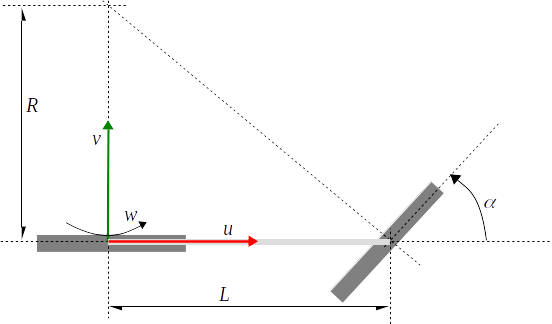
\includegraphics[width=1.0\columnwidth]{figures/bike_kinematics.png}
    \caption{Bicycle configuration.}
    \label{fig:bike_kinematics}
  \end{center}
\end{figure}
Actuator inputs are rear wheel rotation rate, $\Omega$, and front wheel steering angle, $\alpha$. Constructive parameters are the distance between wheels ,$L$, and the rear wheel radius, $r$. Parameter $R$ in the figure~\ref{fig:bike_kinematics} is the curvature radius, which is an intermediate parameter of ineterst.

The linear velocities are: 
\begin{align}
\label{eq:bike_fwd_kinematics_1}
u = \Omega r \\
v = 0
\end{align} 
and the vehicle should fulfill:
\begin{equation}
 u = wR.
\end{equation}
Given 
\begin{equation}
 \tan \alpha = \frac{L}{R}
\end{equation}
and matching the two previous expressions for $u$:
\begin{equation}
 u = \Omega r = wR = w\frac{L}{\tan \alpha} 
\end{equation}
leads to the expression for vehicle rotation rate: 
\begin{equation}
\label{eq:bike_fwd_kinematics_2}
w=\frac{\Omega r}{L} \tan \alpha 
\end{equation}

In this case the forward kinematics is not linear, since the $w$ part of the twist involve a $\tan()$ relation with the input parameter $\alpha$. 

For several purposes it might be interesting to linearize this relation between input actuators, constructive parameters and output twist(see section~\ref{sec:Linearization} for linearization overview). Starting with the linearization with respect to the input actuators~$\alpha$ and~$\Omega$, the Jacobian is: 
\begin{equation}
\mathbf{J}_{\alpha \Omega} = 
\left[
 \begin{array}{cc}
  0 & r  \\
  0 & 0  \\
  \frac{\Omega r}{L \cos ^2 \alpha} & \frac{r}{L}\tan \alpha
 \end{array}
 \right]; \\ 
\end{equation}
 so forward kinematics relation can be approximated by the linearization as follows: 
\begin{equation}
 \left[
 \begin{array}{c}
  u \\
  v  \\
  w 
 \end{array}
 \right] \approx \mathbf{J}_{\alpha \Omega}
 \left[
 \begin{array}{c}
  \alpha \\
  \Omega \\
 \end{array} 
 \right]
\end{equation}
which can be useful, for instance, for Kalman filtering (see section~\ref{sec:KalmanFilter}).

If the interest is to analyze how sensitive is the kinematics to the constructive parameters, the goal is to compute the Jacobian matrix with respect to the parameters~$r$ and~$L$, and perform an error propagation analysis. First the linearized relation is: 
\begin{equation}
\mathbf{J}_{r L} = 
\left[
 \begin{array}{cc}
  \Omega & 0  \\
  0 & 0  \\
  \frac{\Omega}{L}\tan \alpha & -\frac{\Omega r}{L^2}\tan \alpha
 \end{array}
 \right]; \\ 
\end{equation}
Given an uncertainty in the ~$r$ and~$L$ parameters, represented with a covariance matrix as:
\begin{equation}
\mathbf{C}_{r L} = 
\left[
 \begin{array}{cc}
  \sigma^2_r & 0  \\
  0 & \sigma^2_L  \\
 \end{array}
 \right]; \\ 
\end{equation}
the propagation of such uncertainty to twist space is: 
\begin{equation}
\mathbf{C}_{uvw} = \mathbf{J}_{r L} \mathbf{C}_{r L} \mathbf{J}_{r L}^T = 
 \left[
 \begin{array}{cc}
  \Omega & 0  \\
  0 & 0  \\
  \frac{\Omega}{L}\tan \alpha & -\frac{\Omega r}{L^2}\tan \alpha
 \end{array}
 \right]
 \left[
 \begin{array}{cc}
  \sigma^2_r & 0  \\
  0 & \sigma^2_L  \\
 \end{array}
 \right]
 \left[
 \begin{array}{ccc}
  \Omega & 0 & \frac{\Omega}{L}\tan \alpha\\
  r & 0 & -\frac{\Omega r}{L^2}\tan \alpha
 \end{array}
 \right];
\end{equation}
\begin{equation}
\mathbf{C}_{uvw} = 
 \left[
 \begin{array}{ccc}
  \sigma^2_r \Omega^2 & 0 & \sigma^2_r \frac{\Omega^2}{L}\tan \alpha\\
  0 & 0 & 0\\
  \sigma^2_r \frac{\Omega^2}{L}\tan \alpha & 0 & \frac{\Omega^2}{L^2}\tan^2 \alpha (\sigma^2_r+\frac{r^2}{L^2} \sigma^2_L )
 \end{array}
 \right];
\end{equation}
Meaning that for a reasonable uncertainty values of $\sigma^2_r=10^{-6}\ m^2$ and $\sigma^2_L=10^{-6}\ m^2$ ($1\ mm$ of standard deviation in both cases~$r$ and~$L$), and evaluating at~$\Omega=2\pi\ rad/s$,~$\alpha=45^o$,~$r=0.4\ m$ and~$L=1\ m$, the standard deviations in linear speed and rotational rate of the vehicle are: 
\begin{equation}
 \sigma_u \approx 6\ mm/s ; \ \ \ \sigma_w \approx 4\ mrad/s ;
\end{equation}


\paragraph{Inverse kinematics}
Inverse kinematics for the bicycle configuration is found from equations~\ref{eq:bike_fwd_kinematics_1} and~\ref{eq:bike_fwd_kinematics_2} as follows: 
\begin{align}
 \Omega & = \frac{u}{r} \\
 \alpha & = \arctan(L\frac{w}{u}), \ \ \alpha \in [-\pi/2,\pi/2]
\end{align}


\subsection{Tricycle}
The tricycle has two configurations, depending if the drive actuator is at the front axis or at the back one. In the former configuration, the kinematics relation is exactly those previously analyzed for the monocycle case. However, in the later configuration, the driving actuator is attached at the rear axis, providing a forward velocity, while the front wheel just steers the vehicle. So, this configuration is like the bicycle case analyzed above, but some extra differential mechanism is required to drive each rear wheel at different speeds when turning, otherwise the wheels would slip. 


\subsection{Two wheels differential drive}
Two wheels differential drive configuration is an essential and widely used architecture, due to its building simplicity and good manoeuvring properties, since it allows the platform to turn on the spot. 

Figure~\ref{fig:differential_kinematics} shows the two wheels differential drive configuration as well as the involved parameters and variables. 
\begin{figure}[bth!]
  \begin{center}
    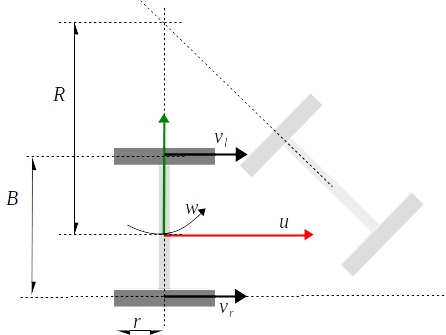
\includegraphics[width=1.0\columnwidth]{figures/differential_kinematics.png}
    \caption{Two wheels differential drive configuration.}
    \label{fig:differential_kinematics}
  \end{center}
\end{figure}

Actuator inputs are left and right wheel rotation rates, $\Omega_l, \Omega_r$. Constructive parameters are the baseline distance between wheels ,$B$, and the wheel radius, $r$. Parameter $R$ in the figure~\ref{fig:differential_kinematics} is the curvature radius, which is an intermediate parameter of ineterst.

Placing the platform frame at the mid point on the baseline joining the wheels, we define the twist of this frame as $(u, v, w)$. Applying the Coriolis principle, three equations are deduced, for the left wheel center point, the right wheel center point and the vehicle origin, respectively:
\begin{align}
v_l = & \Omega_l r = w(R-\frac{B}{2}) \\
v_r = & \Omega_r r = w(R+\frac{B}{2}) \\
u = & wR \\
\end{align} 
operating on $v_r-v_l$, leads to:
\begin{equation}
\label{eq:diff_drive_fwd_kinematics_w}
w = \frac{v_r-v_l}{B}
\end{equation}
and solving for $v_r+v_l$, the linear forward velocity is:  
\begin{equation}
\label{eq:diff_drive_fwd_kinematics_u}
u = \frac{v_r+v_l}{2}
\end{equation}

In this case the kinematics relation between actuators and platform twist is linear, and can be written in the matrix form:
\begin{equation}
\label{eq:diff_drive_fwd_kinematics_matrix}
 \left[
 \begin{array}{c}
  u \\
  w \\
 \end{array}
 \right] = 
 \left[
 \begin{array}{cc}
  \frac{1}{2} & \frac{1}{2} \\
  -\frac{1}{B} & \frac{1}{B} \\
 \end{array}
 \right]
 \left[
 \begin{array}{c}
  v_l \\
  v_r \\
 \end{array}
 \right] = 
 \left[
 \begin{array}{cc}
  \frac{r}{2} & \frac{r}{2} \\
  -\frac{r}{B} & \frac{r}{B} \\
 \end{array}
 \right]
 \left[
 \begin{array}{c}
  \Omega_l \\
  \Omega_r \\
 \end{array}
 \right]
\end{equation}

As in the bicycle case (see subsection \ref{subsec:bicycle}), we might be interested how errors on constructive parameters~$r$ and~$B$ propagate to the platform twist. In this case the Jacobian of the twist with respect to these parameters is computed as: 
\begin{equation}
\mathbf{J}_{r B} = 
\left[
 \begin{array}{cc}
  \frac{1}{2}(\Omega_r+\Omega_l) & 0  \\
  \frac{1}{B}(\Omega_r-\Omega_l) & \frac{r}{B^2}(\Omega_l-\Omega_r)  \\
 \end{array}
 \right]; \\ 
\end{equation}
Given an uncertainty in the ~$r$ and~$B$ parameters, represented with a covariance matrix as:
\begin{equation}
\mathbf{C}_{r B} = 
\left[
 \begin{array}{cc}
  \sigma^2_r & 0  \\
  0 & \sigma^2_B  \\
 \end{array}
 \right]; \\ 
\end{equation}
the propagation of such uncertainty to twist space is: 
\begin{equation}
\mathbf{C}_{uw} = \mathbf{J}_{r B} \mathbf{C}_{r B} \mathbf{J}_{r B}^T = 
 \left[
 \begin{array}{cc}
 \frac{\sigma^2_r}{4}(\Omega_r+\Omega_l)^2 & \frac{\sigma^2_r}{4}(\Omega_r+\Omega_l)(\Omega_r-\Omega_l) \\
 \frac{\sigma^2_r}{4}(\Omega_r+\Omega_l)(\Omega_r-\Omega_l) & \frac{\sigma^2_r}{4}(\Omega_r-\Omega_l)^2 + \frac{\sigma^2_B r^2}{B^4}(\Omega_l-\Omega_r)^2 \\
 \end{array}
 \right];
 \label{eq:differential_twist_uncertainty}
\end{equation}
Result in equation~\ref{eq:differential_twist_uncertainty} suggests that error in baseline length~$B$ only affects the uncertainty of the platform rotation rate, while errors in wheel radius~$r$ propagates to both components of the twist~$u$ and ~$w$. 

\paragraph{Inverse kinematics}
Inverse kinematics for the two wheels differential configuration can be derived by inverting the linear model in equation~\ref{eq:diff_drive_fwd_kinematics_matrix}, or from equations~\ref{eq:diff_drive_fwd_kinematics_u} and~\ref{eq:diff_drive_fwd_kinematics_w}: 
\begin{align}
\label{eq:diff_drive_inv_kinematics}
 v_r & = u + w\frac{B}{2} \\
 v_l & = u - w\frac{B}{2} \\
\end{align}
which suggests that for positive rotations, the right wheel should turn faster than the left one.

\subsection{4 wheels differential drive}
At kinematics level, this configuration reduces to the case of two wheel differential drive since both left wheels have the same rotation rate and both right wheels have also the same rotation rate. However, when the vehicle is rotating, null lateral velocity at wheels is no longer fulfilled, so the wheels slip when turning. 


\subsection{Ackermann}
Ackermann system is the standard steering for most of the nowadays cars and trucks. Figure~\ref{fig:ackermann_kinematics} shows the steering mechanism, the constructive parameters~$B$ and~$L$ and the input actuators~$\alpha$ and~$u$, the later being directly the forward velocity to be transmitted to each rear wheel.  
\begin{figure}[bth!]
  \begin{center}
    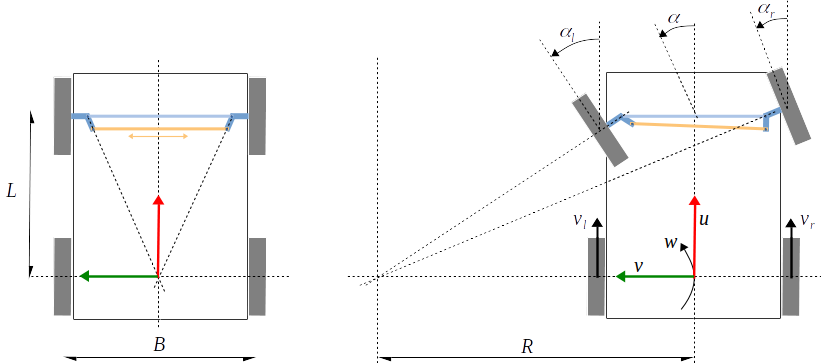
\includegraphics[width=1.0\columnwidth]{figures/ackermann_kinematics.png}
    \caption{Ackermann configuration. Steering is achieved by actuating the orange bar.  }
    \label{fig:ackermann_kinematics}
  \end{center}
\end{figure}

The kinematics of the Ackermann configuration is reduced to the kinematics of the bike seen at subsection~\ref{subsec:bicycle}, with input actuators~$\alpha$ and~$u$, and constructive parameter~$L$.

However, the Ackermann mechanism ensures a relation between the three steering angles~$\alpha_l$, $\alpha_r$ and~$\alpha$. Given an steering angle~$\alpha$, the tangent of the three triangles with vertex at ICR are: 
\begin{align}
\tan \alpha_l = & \frac{L}{R-\frac{B}{2}} \\
\tan \alpha = & \frac{L}{R} \\
\tan \alpha_r = & \frac{L}{R+\frac{B}{2}} 
\end{align} 
Solving for~$R$ at each equation leads to the following relation that Ackemrann steering should fulfill: 
\begin{align}
\tan \alpha_l = & \frac{1}{\frac{1}{\tan \alpha} - \frac{B}{2L}} \\
\tan \alpha_r = & \frac{1}{\frac{1}{\tan \alpha} + \frac{B}{2L}} \\\end{align} 
which is of interest in case of electronic Ackermann steering. 

Even if forward velocity~$u$ is transmitted to each rear wheel,  velocities of each of these wheels are different and constrained with the vehicle twist. Usually a differential mechanism implements this difference of speeds, but an electronic implementation may implement that, fulfilling the following: 
\begin{align}
v_l = & w(R-\frac{B}{2}) \\
v_r = & w(R+\frac{B}{2})
\end{align} 
which as it has been seen with the two wheel differential drive at equations~\ref{eq:diff_drive_inv_kinematics}, it leads to: 
\begin{align}
v_l = & u -w\frac{B}{2} \\
v_r = & u + w\frac{B}{2}
\end{align} 



\subsection{Double Ackermann}
Double Ackermann configuration refers to those vehicles having an Ackermann steering system (mechanical or electronical) for front and back wheels, actuating both with the same steering angle, so the ICR point is no longer at the line joining rear wheels , but it is at the line parallel to that but passing through the center of the vehicle. This allows such vehicles to make sharper turns than single Ackermann steering configurations. The configuration of double Ackermann steering can be reduced to a bicycle with  steering at front and back wheels, as shown in figure~\ref{fig:double_ackermann_kinematics}.
\begin{figure}[bth!]
  \begin{center}
    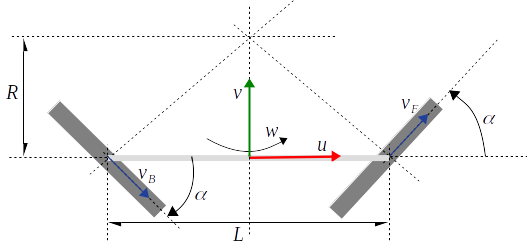
\includegraphics[width=1.0\columnwidth]{figures/double_ackermann_kinematics.png}
    \caption{Double Ackermann configuration can be reduced to the double steering bike.}
    \label{fig:double_ackermann_kinematics}
  \end{center}
\end{figure}

The analysis of this double steering bicycle starts by applying the Coriols principle at the center of each wheel, as well as at the center of the bicycle:
\begin{align}
\mathbf{v_B} = & 
\left[
 \begin{array}{c}
  0  \\
  0  \\
  w 
 \end{array}
\right]
\times 
\left[
 \begin{array}{c}
  -\frac{L}{2}  \\
  -R  \\
  0 
 \end{array}
\right]
= 
\left[
 \begin{array}{c}
  wR  \\
  -w\frac{L}{2}  \\
  0 
 \end{array}
\right] \\
\mathbf{u} = & 
\left[
 \begin{array}{c}
  0  \\
  0  \\
  w 
 \end{array}
\right]
\times 
\left[
 \begin{array}{c}
  0  \\
  -R  \\
  0 
 \end{array}
\right]
= 
\left[
 \begin{array}{c}
  wR  \\
  0  \\
  0 
 \end{array}
\right] \\
\mathbf{v_F} = & 
\left[
 \begin{array}{c}
  0  \\
  0  \\
  w 
 \end{array}
\right]
\times 
\left[
 \begin{array}{c}
  \frac{L}{2}  \\
  -R  \\
  0 
 \end{array}
\right]
= 
\left[
 \begin{array}{c}
  -wR  \\
  w\frac{L}{2}  \\
  0 
 \end{array}
\right]
\end{align} 
The above velocity vectors~$\mathbf{v_B}$, $\mathbf{u}$ and~$\mathbf{v_F}$ are expressed with respect to a frame placed at ICR and aligned with the vehicle frame, so the same velocity vectors are also with respect to the vehicle frame (since there is no rotation between these two frames). For the back wheel, in 2D, we have: 
\begin{equation}
\mathbf{v_B} = 
\left[
 \begin{array}{c}
  wR  \\
  -w\frac{L}{2} 
 \end{array}
\right]
=
|\mathbf{v_B}|
\left[
 \begin{array}{c}
  \cos \alpha  \\
  \sin \alpha
 \end{array}
\right]
=
\Omega_Br
\left[
 \begin{array}{c}
  \cos \alpha  \\
  \sin \alpha
 \end{array}
\right]
\end{equation}
so we can find $R$ and $w$ as: 
\begin{align}
 R = & \frac{\Omega_B r}{w}\cos \alpha \\
 w = & \frac{2\Omega_B r}{L}\sin \alpha \\
\end{align}
and then, with the expression of $\mathbf{u}=\left[u_x\ u_y \right]^T$ in 2D: 
\begin{equation}
 u_x = wR = \Omega_Br \cos \alpha \ ; \ \ u_y = 0; 
\end{equation}

A practical case of double Ackermann steering (or even more than double!) is the straddle carrier family (see figure~\ref{fig:straddle_carrier}), which are large vehicles that need to manoeuver usually in tight spaces with respect to their dimensions~$L$ and~$B$. 
\begin{figure}[bth!]
  \begin{center}
    \includegraphics[width=0.6\columnwidth]{figures/straddle_carrier.jpg}
    \caption{Straddle carriers are big vehicles that need to perform good manoeuvring, so they have double (or even quadruple like in this picture) Ackermann steering, usually implemented with electronic/software means instead of by a mechanism.}
    \label{fig:straddle_carrier}
  \end{center}
\end{figure}


\subsection{Holonomic wheels}
Holonomic wheels refers to those wheels that have an extra set of small rollers mounted with their axis forming an angle $\gamma$ with the wheel perpendicular direction of driving. This angle $\gamma$ is usually $0$~degrees for \textit{omniwheels} or $45$~degrees for \textit{mecanum} wheels. These rollers allow the wheel to freely move in lateral motion, while keeping the actuated forward (standard) motion of a wheel, so the constraint of null lateral motion described in~\ref{subsec:single_wheel} no longer fulfills. 

Figure\ref{fig:omniwheel_kinematics} shows the involved frames and vectors to analyze the inverse kinematics of an omniwheel mounted in a vehicle frame.
\begin{figure}[bth!]
  \begin{center}
    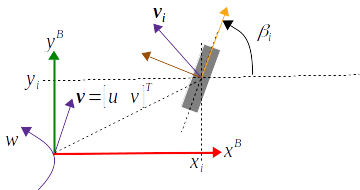
\includegraphics[width=1.0\columnwidth]{figures/omniwheel_kinematics.png}
    \caption{Frames and vectors involved in the omniwheel kinematcs analysis. Vehicle frame in green and red. In yellow wheel driving direction and in brown wheel free sliding direction for omniwheels. }
    \label{fig:omniwheel_kinematics}
  \end{center}
\end{figure}

Given a vehicle twist~$[u v w]$, the procedure will find the inverse kinematics model, so the required wheel angular speeds for each wheel. The first step is to find the linear velocity of the wheel center with respect to the vehicle base frame~$\mathcal{F}^B$, given the vehicle twist, by applying the Coriolis law: 
\begin{equation}
\mathbf{v^B_i} = 
\left[
 \begin{array}{c}
  u  \\
  v \\
  0
 \end{array}
\right]
+
\left[
 \begin{array}{c}
  0  \\
  0 \\
  w
 \end{array}
\right]
\times
\left[
 \begin{array}{c}
  x_i \\
  y_i
 \end{array}
\right] 
= 
\left[
 \begin{array}{c}
  u  \\
  v \\
  0
 \end{array}
\right]
+
\left[
\begin{array}{c}
 -w y_i \\
 w x_i \\
 0
\end{array}
\right] 
= 
\left[
\begin{array}{ccc}
 1 & 0 & -y_i \\
 0 & 1 &  x_i 
\end{array}
\right] 
\left[
\begin{array}{c}
 u \\
 v \\
 w
\end{array}
\right] 
\end{equation}

Once we know the wheel center linear speed with respect to the vehicle frame, we will transform it to the wheel frame by applying the rotation (only the 2D part): 
\begin{equation}
\mathbf{v^{W}_i} = 
\left[
 \begin{array}{cc}
  \cos \beta_i & \sin \beta_i  \\
  -\sin \beta_i & \cos \beta_i \\
 \end{array}
\right]
\left[
\begin{array}{ccc}
 1 & 0 & -y_i \\
 0 & 1 &  x_i 
\end{array}
\right] 
\left[
\begin{array}{c}
 u \\
 v \\
 w
\end{array}
\right] 
\end{equation}

Finally, from~$\mathbf{v^{W}_i}$, we only take the first component, which is the actuated velocity (aligned with the wheel driving direction): 
\begin{equation}
u_i
=
\left[
\begin{array}{cc}
 1 & 0
\end{array}
\right]
\left[
 \begin{array}{cc}
  \cos \beta_i & \sin \beta_i  \\
  -\sin \beta_i & \cos \beta_i \\
 \end{array}
\right]
\left[
\begin{array}{ccc}
 1 & 0 & -y_i \\
 0 & 1 &  x_i 
\end{array}
\right] 
\left[
\begin{array}{c}
 u \\
 v \\
 w
\end{array}
\right] 
\end{equation}
which can be simplified to: 
\begin{equation}
u_i 
=
\left[
\begin{array}{ccc}
 \cos \beta_i & \sin \beta_i & -y_i\cos \beta_i+x_i \sin \beta_i
\end{array}
\right]
\left[
\begin{array}{c}
 u \\
 v\\
 w
\end{array}
\right]
\label{eq:single_omniwheel_inverse_kniematics}
\end{equation}

A vehicle with $N$ omniwheels (at least $N=3)$, will stack $N$ equations that constraint the actuated wheel angular speeds given the vehicle twist. The following subsections analyses the cases for $N=3$ and $N=4$. 


\subsection{4 omniwheels}
The four omniwheels configuration is a rather standard platform allowing high manoeuvrability and stability. Figure~\ref{fig:four_omniwheels_kinematics} shows this configuration when mounted in a squared platform of side size $2L$.
\begin{figure}[bth!]
  \begin{center}
    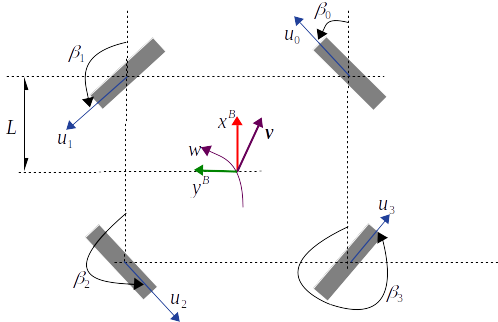
\includegraphics[width=1.0\columnwidth]{figures/four_omniwheels_kinematics.png}
    \caption{Configuration for a platform with four omniwheels in a square base of side size $2L$.}
    \label{fig:four_omniwheels_kinematics}
  \end{center}
\end{figure}

Table~\ref{tab:params_4_omni} details the constructive parameters~$x_i,y_i,B_i$ for this vehicle. 
\begin{table}[hbt] \centering
\caption{Constructive parameters for squared 4-omniwheel vehicle of side size $2L$}
\begin{tabular}
[c]{|c|c|c|c|}\hline
		& $x_i$ 		& $y_i$				& $\beta_i$ \\\hline
Wheel 0 & $L$ 		    & $-L$				& $\pi/4$ \\\hline
Wheel 1 & $L$ 		    & $L$				& $3\pi/4$ \\\hline
Wheel 2 & $-L$ 		    & $L$				& $5\pi/4$ \\\hline
Wheel 3 & $-L$ 		    & $-L$				& $7\pi/4$ \\\hline
\end{tabular}
\label{tab:params_4_omni}
\end{table}

With the constructive parameters, wheel actuated speeds can be computed by applying equation~\ref{eq:single_omniwheel_inverse_kniematics} for each wheel ($i=0,..,3$):
\begin{equation}
\left[
\begin{array}{c}
u_0 \\
u_1 \\
u_2 \\
u_3 \\
\end{array}
\right]
=
\left[
\begin{array}{ccc}
 \cos \beta_0 & \sin \beta_0 & -y_0\cos \beta_0+x_0 \sin \beta_0 \\
 \cos \beta_1 & \sin \beta_1 & -y_1\cos \beta_1+x_1 \sin \beta_1 \\
 \cos \beta_2 & \sin \beta_2 & -y_2\cos \beta_2+x_2 \sin \beta_2 \\
 \cos \beta_3 & \sin \beta_3 & -y_3\cos \beta_3+x_3 \sin \beta_3 \\
\end{array}
\right]
\left[
\begin{array}{c}
 u \\
 v\\
 w
\end{array}
\right], 
\end{equation}

so the full inverse kinematics results as follows: 
\begin{equation}
\left[
\begin{array}{c}
u_0 \\
u_1 \\
u_2 \\
u_3 \\
\end{array}
\right]
=
\left[
\begin{array}{ccc}
 \frac{1}{\sqrt{2}} & \frac{1}{\sqrt{2}} & L\sqrt{2} \\
 -\frac{1}{\sqrt{2}} & \frac{1}{\sqrt{2}} & L\sqrt{2} \\
 -\frac{1}{\sqrt{2}} & -\frac{1}{\sqrt{2}} & L\sqrt{2} \\
 \frac{1}{\sqrt{2}} & -\frac{1}{\sqrt{2}} & L\sqrt{2} \\
\end{array}
\right]
\left[
\begin{array}{c}
 u \\
 v\\
 w
\end{array}
\right], 
\end{equation}

Please remind that $u_i$ are the linear speeds of wheel centers in the driving direction. To find the angular speed of the wheel we have to apply $\Omega_i = u_i/r$, where $r$ is the radius of the wheel. 


\subsection{3 omniwheels}
A typical configuration using omniwheels is also that of mounting three of them in an equilateral triangle base, as depicted in figure~\ref{fig:three_omniwheels_kinematics}.
\begin{figure}[bth!]
  \begin{center}
    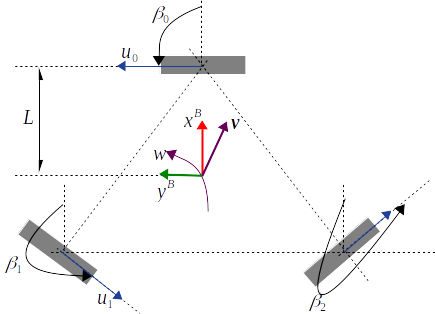
\includegraphics[width=1.0\columnwidth]{figures/three_omniwheels_kinematics.png}
    \caption{Configuration for a platform with three omniwheels in an equilateral triangle.}
    \label{fig:three_omniwheels_kinematics}
  \end{center}
\end{figure}

In this case table~\ref{tab:params_3_omni} shows the constructive parameters  $x_i,y_i,\beta_i$: 
\begin{table}[hbt] \centering
\caption{Constructive parameters for triangular 3-omniwheel vehicle of side size $2L$}
\begin{tabular}
[c]{|c|c|c|c|}\hline
		& $x_i$ 		    & $y_i$				& $\beta_i$ \\\hline
Wheel 0 & $L$ 		        & $0$				& $3\pi/6$ \\\hline
Wheel 1 & $-L\sin(\pi/6)$   & $L\cos(\pi/6)$	& $7\pi/6$ \\\hline
Wheel 2 & $-L\sin(\pi/6)$ 	& $-L\cos(\pi/6)$	& $11\pi/4$ \\\hline
\end{tabular}
\label{tab:params_3_omni}
\end{table}

Therefore, applying equation~\ref{eq:single_omniwheel_inverse_kniematics}, the inverse kinematics results in the following: 
\begin{equation}
\left[
\begin{array}{c}
u_0 \\
u_1 \\
u_2 \\
\end{array}
\right]
=
\left[
\begin{array}{ccc}
 0      & 1     & L \\
-\frac{\sqrt{3}}{2} & -\frac{1}{2} & L \\
 \frac{\sqrt{3}}{2} & -\frac{1}{2} & L \\
\end{array}
\right]
\left[
\begin{array}{c}
 u \\
 v \\
 w
\end{array}
\right]
\end{equation}



\subsection{4 mecanum wheels}


\subsection{Dynamics}





\newpage
\part{Estimation}

\newpage
\section{Least Squares}
The first three subsections of this section get inspiration from the book~\cite{simon06}, which explains the linear least squares topic in three gradual steps, to finally introduce the Kalman Filter in a natural and smooth way. The same approach is followed in this section, by first presenting the Linear Least Squares, thereafter the Weighted Linear Least Squares and then the Recursive approach. The fourth subsection is devoted to non-linear least squares topic.

The underlying idea and goal of the Least Squares topic is to \textit{find the system state that better explain your measurements}.

\subsection{Unweighted Linear Least Squares (UL-LS)}
Let be $\mathbf{x} \in \mathbb{R}^n$ the system state of~$n$ components, and~$\mathbf{z} \in \mathbb{R}^m$ a set of~$m$ measurements. Assuming the following linear model for the measurements:
\begin{equation}
 \mathbf{z} = \mathbf{H}\mathbf{x} + \mathbf{n}_z
\end{equation}
The goal of the Least Squares procedure is to estimate the state~$\mathbf{x}$ that better explain the measurements~$\mathbf{z}$. The problem in the above equation is that the true values of the noise~$\mathbf{n}_z$ for each measurement (each component) in~$\mathbf{z_i}$ are unknown. However, the noise is assumed to be a random variable following a normal distribution:
\begin{equation}
 \mathbf{n}_z \approx \mathcal{N}(0,\sigma^2_{n_z}\mathbf{I})
\end{equation}
so all the measurements are independent and have the same distribution, since the covariance matrix is an identity multiplied by a constant~$\sigma_{n_z}$.
We can define the \textit{expected measurement} vector as:
\begin{equation}
 \hat{\mathbf{z}} = \mathbf{H}\mathbf{x}
\end{equation}
which is the measurements we expect, according the model and given the state~$\mathbf{x}$. A measurement error can be also defined as: 
\begin{equation}
 \mathbf{e}_z = \mathbf{z} - \hat{\mathbf{z}}
\end{equation}
Given this error, the squared norm of it (squared length) seems to be an appropriate indicator to evaluate how big is this error, so it is defined the following function as the squared norm of the measurement error:
\begin{equation}
 f(\mathbf{e}_z) = \mathbf{e}^T_z\mathbf{e}_z = \sum^m_{i=1}e^2_i
\end{equation}
The criterion to find the state estimate,~$\hat{\mathbf{x}}$, that better explains the measurements is, therefore, to find those state~$\mathbf{x}$ that minimizes the function~$f(\mathbf{e}_z)$, so that minimizes the length of the error vector.
\begin{equation}
 \hat{\mathbf{x}} = \operatorname*{arg\,min}_{\mathbf{x}}\ f(\mathbf{e}_z)
\end{equation}
Developping the  expression of~$f(\mathbf{e}_z)$ to show explicitly its dependency on~$\mathbf{x}$:
\begin{equation}
 f(\mathbf{e}_z) = \mathbf{e}^T_z\mathbf{e}_z = (\mathbf{z}-\hat{\mathbf{z}})^T (\mathbf{z}-\hat{\mathbf{z}})
		 = (\mathbf{z}-\mathbf{H}\mathbf{x})^T(\mathbf{z}-\mathbf{H}\mathbf{x})
		 = \mathbf{z}^T\mathbf{z} - \mathbf{z}^T\mathbf{H}\mathbf{x} - \mathbf{x}^T\mathbf{H}^T\mathbf{z} + \mathbf{x}^T\mathbf{H}^T\mathbf{H}\mathbf{x}
\end{equation}
and then, forcing the derivative with respect to~$\mathbf{x}$ to be~$0$ to find the minimum:
\begin{equation}
  \frac{\partial f(\mathbf{e}_z)}{\partial \mathbf{x}} 
	= -\mathbf{z}^T\mathbf{H} -\mathbf{z}^T\mathbf{H} + 2\mathbf{x}^T\mathbf{H}^T\mathbf{H} = 0;
  \ \ \mathbf{x}^T\mathbf{H}^T\mathbf{H} = \mathbf{z}^T\mathbf{H};
  \ \ \mathbf{H}^T\mathbf{H}\mathbf{x} = \mathbf{H}^T\mathbf{z};
\end{equation}
and solving for~$\mathbf{x}$, we finally get the optimal state estimate as:
\begin{equation}
\label{eq:ul_least_squares}
 \hat{\mathbf{x}} = (\mathbf{H}^T\mathbf{H})^{-1}\mathbf{H}^T\mathbf{z}
\end{equation}
which provides an estimate of the state, given all the measurements~$\mathbf{z}$, a linear measurement model~$\mathbf{H}$, according to the criterion of minimal measurement error, and assuming all measurements have independent noise, but they follow the same normal distribution. 

\subsection{Weighted Linear Least Squares (WL-LS)}
In case we have a different confidence level for each measurement. Instead of throwing away the most uncertain measurements, it is wise to also use it, but \textit{weight} them less than the most certain ones. Moreover, some measurements can experience some level of covariance between them. The same linear measurement model than the one used in the unweighted case is assumed here:
\begin{equation}
 \mathbf{z} = \mathbf{H}\mathbf{x} + \mathbf{n}_z
\end{equation}
but in the weighted case, the measurement noise covariance can be a generic covariance matrix:
\begin{equation}
 \mathbf{n}_z \approx \mathcal{N}(0,\mathbf{C}_{n_z})
\end{equation}
The goal of the Weighted Least Squares procedure is to estimate the state~$\mathbf{x}$ that better explain the measurements~$\mathbf{z}$, taking into account different confidence levels for each of them.

To derive the final equation, a procedure similar to previous subsection is adopted, but in this case the function~$f(\mathbf{e}_z)$ to be minimized is the weighted norm, which can be interpreted as the Mahalanobis distance of the measurement error vector~$\mathbf{e}_z$ to the origin:
\begin{equation}
 f(\mathbf{e}_z) = \mathbf{e}^T_z\mathbf{C}^{-1}_{n_z}\mathbf{e}_z
\end{equation}
Imposing the same criterion of minimizing function~$f(\mathbf{e}_z)$ with respect to~$\mathbf{x}$, we get: 
\begin{equation}
 \frac{\partial f(\mathbf{e}_z)}{\partial \mathbf{x}} = 
 -\mathbf{z}^T\mathbf{C}^{-1}_{n_z}\mathbf{H} + \mathbf{x}^T\mathbf{H}^T\mathbf{C}^{-1}_{n_z}\mathbf{H} = 0; 
\end{equation}
and solving, the optimal state estimate is finally computed as:
\begin{equation}
\label{eq:wl_least_squares}
 \hat{\mathbf{x}} = (\mathbf{H}^T\mathbf{C}^{-1}_{n_z}\mathbf{H})^{-1}\mathbf{H}^T\mathbf{C}^{-1}_{n_z}\mathbf{z}
\end{equation}

\subsection{Recursive Weighted Linear Least Squares (RWL-LS)}
\label{subsec:recursive_ls}
The two previous subsections compute the state estimate~$\hat{\mathbf{x}}$ once all the measurements were available. This is usually called \textit{batch} mode, when you solve a problem off-line with all the measurements took into account in one single step. But real robotic estimation processes usually receive measurements one by one, since they usually come from some sensor source or detector process. Solving at each iteration the entire problem from the beginning would produce huge measurement vectors~$\mathbf{z}$ after a while, but even more critical, untreatable covariance matrices~$\mathbf{H}$ and~$\mathbf{C}_{n_z}$ to be inverted. So it is important to find a recursive approach to solve a linear least squares in such context. 

At a given iteration~$t$, we continue to assume a linear measurement model, which \textit{may} change at each iteration, as it is indicated with the~${}^t$ superindex: 
\begin{equation}
 \mathbf{z}^t = \mathbf{H}^t\mathbf{x}^t + \mathbf{n}^t_z,
\end{equation}
but now, a linear system model is also proposed which recursively updates the current state, based on the previous one: 
\begin{equation}
 \mathbf{x}^t = \mathbf{x}^{t-1} + \mathbf{K}^t(\mathbf{z}^t - \mathbf{H}^t\mathbf{x}^{t-1}).
\end{equation}
Given an initialization of~$\mathbf{x}^0$, right-sides of both equations above are known, exceptuating the matrix~$\mathbf{K}^t$, called the \textit{gain}, and the particular values of the mesurement noise in a given iteration,~$\mathbf{n}^t_z$. However the noise distribution is assumed to be known, as we did in the non-recursive case. In order to derive the final set of equations for the recursive algorithm, the goal is to find this gain matrix~$\mathbf{K}^t$. In that case, the criterion will change, and it will be to minimize the sum of the variances of the estimation error at iteration~$t$. So the function to minimize is:
\begin{equation}
 f(\mathbf{e}^t_x) = Tr\{\mathbf{C}^t_{x}\},
\end{equation}
where the operator $Tr\{\}$ is the trace of the matrix, which is the sum of all diagonal elements (variances) of the covariance matrix. Expressing the estimation error as: 
\begin{equation}
 \mathbf{e}^t_x = \mathbf{x}^t - \hat{\mathbf{x}}^t
\end{equation}
so the covariance matrix, by definition is the expectation of $\mathbf{e}_x\mathbf{e}^T_x$:
\begin{equation}
 \mathbf{C}^t_{x} = \mathcal{E}\{\mathbf{e}^t_x(\mathbf{e}^t_x)^T\}
\end{equation}
which after some maths (see~\cite{simon06}), leads to: 
\begin{equation}
 \mathbf{C}^t_{x} = (\mathbf{I}-\mathbf{K}^t\mathbf{H}^t)\mathbf{C}^{t-1}_x(\mathbf{I}-\mathbf{K}^t\mathbf{H}^t)^T
		    + \mathbf{K}^t\mathbf{C}^t_{n_z}(\mathbf{K}^t)^T
\end{equation}
Coming back to our minimization goal, 
\begin{equation}
 f(\mathbf{e}^t_x) = Tr\{\mathbf{C}^t_{x}\} \rightarrow \frac{\partial f(\mathbf{e}^t_x)}{\partial \mathbf{K}^t} = 0
\end{equation}
which finishes with the expression for the gain:
\begin{equation}
 \mathbf{K}^t = \mathbf{C}^{t-1}_x(\mathbf{H}^t)^T(\mathbf{H}^t\mathbf{C}^{t-1}_x(\mathbf{H}^t)^T+\mathbf{C}^t_{n_z})^{-1}
\end{equation}

The algorithm~\ref{alg:recursive_ls} summarizes all the steps for the recursive least squares approach. The algorithm requires three inputs to start looping: the initial guess for the state estimate,~$\mathbf{x}^0$, the initial guess for the covariance of the state estimate,~$\mathbf{C}^0_x$, and the measurement model,~$\mathbf{H}^t$ which may, or may not, be time dependent. The algorithm provides at the end of each iteration~$t$ the state estimate that better explain the measurements received up to~$t$, according the criterion of minimizing the trace of~$\mathbf{C}^t_x$.
\begin{algorithm}
\caption{Recursive Weighted Linear Least Squares}
INPUTS: $\hat{\mathbf{x}}^0,\mathbf{C}^0_x,\mathbf{H}^t,\mathbf{C}^t_{n_z}$\\
OUTPUT: $\hat{\mathbf{x}}^t,\mathbf{C}^t_x$, at each iteration
\begin{algorithmic}
\STATE INIT: $\hat{\mathbf{x}}^0,\mathbf{C}^0_x$
\STATE FOR EACH ITERATION
\STATE \hspace{1cm} $\mathbf{H}^t$ //Compute it, if it is not constant
\STATE \hspace{1cm} $\hat{\mathbf{z}}^t = \mathbf{H}^t\hat{\mathbf{x}}^{t-1}$ //Compute the expected measurement 
\STATE \hspace{1cm} $\mathbf{K}^t = \mathbf{C}^{t-1}_x(\mathbf{H}^t)^T(\mathbf{H}^t\mathbf{C}^{t-1}_x(\mathbf{H}^t)^T+\mathbf{C}^t_{n_z})^{-1}$ 
//Compute the gain
\STATE \hspace{1cm} $\hat{\mathbf{x}}^t = \hat{\mathbf{x}}^{t-1} + \mathbf{K}^t(\mathbf{z}^t - \hat{\mathbf{z}}^t)$ //Update the state estimate
\STATE \hspace{1cm} $\mathbf{C}^t_{x} = (\mathbf{I}-\mathbf{K}^t\mathbf{H}^t)\mathbf{C}^{t-1}_x(\mathbf{I}-\mathbf{K}^t\mathbf{H}^t)^T
		    + \mathbf{K}^t\mathbf{C}^t_{n_z}(\mathbf{K}^t)^T$ //Update the covariance of the state estimate
\RETURN $\hat{\mathbf{x}}^t,\mathbf{C}^t_x$		    
\STATE END FOR
\end{algorithmic}
\label{alg:recursive_ls}
\end{algorithm}

\paragraph{Example \theexamplecounter. Estimate a constant velocity from wheel encoders.}
\stepcounter{examplecounter}
This example assumes a 4-wheeled vehicle running at constant forward velocity~$v$ and rotational rate~$\omega$ on a plane.
We want to estimate these two variables, from the measurements we get from each wheel encoder. So, the main step we have to solve is to find the measurement model, which relates the state~$\mathbf{x}=[v\ \omega]$ with these measurements.
\begin{figure}[h!]
  \includegraphics[width=1\linewidth]{figures/wheel-4diff_kinematics.eps}
  \caption{Differential 4-wheel kinematics: from wheel rotational rates to vehicle linear and rotational velocities~$v,\omega$.}
  \label{fig:wheel-4diff_kinematics}
\end{figure}

The measurements we have are the four linear velocities provided by the four encoders mounted at each wheel axis (see figure~\ref{fig:wheel-4diff_kinematics}). These linear velocities are directly the rotational velocities,~$\omega_w$ reported by each encoder multiplied by the wheel radius,~$r_w$:
\begin{equation}
v_{lf} = \omega_{lf}r_{lf};\ v_{lb} = \omega_{lb}r_{lb};\ v_{rf} = \omega_{rf}r_{rf};\ v_{rb} = \omega_{rb}r_{rb}
\end{equation}
where $\omega_{**}$, $v_{**}$ and~$r_{**}$ are rotational and linear speeds and radius for each wheel (left/right front/back). We consider the radius of the wheels to be precisely known,~$r_w$, so the only random variable is each rotational speed measurement, which leads to random variables at linear speed for each wheel. 

From the kinematics of a 4-wheeled platform (Figure~\ref{fig:wheel-4diff_kinematics}), we have the following two equations, for left and right velocities, according to the rotational rate of the vehicle. These equations relate the arc run by the robot, for the left-wheels and for the right ones, during a $\Delta\tau$ time step:
\begin{equation}
\begin{array}{cc}
 v_l\Delta\tau = & \omega\Delta\tau(r_c+\frac{b}{2}) \\
 v_r\Delta\tau = & \omega\Delta\tau(r_c-\frac{b}{2}) 
\end{array}
\label{eq:v_l_v_r}
\end{equation}
where the curvature radius of the vehicle's trajectory,~$r_c$, is provided by the relation~$v=\omega r_c$. Rearranging terms, we finish with the following two equations which explain measurements~$v_{l*},v_{r*}$ as a function of the system state~$\mathbf{x}=[v\ \omega]^T$
\begin{equation}
\begin{array}{cc}
 v_{l*} = v+\omega\frac{b}{2} \\
 v_{r*} = v-\omega\frac{b}{2}
\end{array}
\end{equation}
so the measurement process is modelled as:
\begin{equation}
 \mathbf{z}^t = \mathbf{H}^t\mathbf{x}^t + \mathbf{n}^t_z 
\end{equation}
where each term of the above equation is:
\begin{equation}
 \mathbf{z}^t =
 \left[
 \begin{array}{c}
  v_{lf}\\
  v_{lb}\\
  v_{rf}\\
  v_{rb}
 \end{array}
 \right]; \ 
 \mathbf{H}^t = \mathbf{H} = 
 \left[
 \begin{array}{cc}
  1 & b/2 \\
  1 & b/2 \\
  1 & -b/2 \\
  1 & -b/2 \\
 \end{array}
 \right];\ 
 \mathbf{x}^t=
 \left[
 \begin{array}{c}
  v\\
  \omega
 \end{array}
 \right]^t;\ 
 \mathbf{n}^t_z \sim \mathcal{N}(\mathbf{0},\mathbf{C}_{n_z})
\end{equation}
At this point, we need to model the measurement noise, by setting the coefficients of the~$\mathbf{C}_{n_z}$ matrix according of data and knowledge we may have coming from the device datasheets and/or the measurement procedures (misscalibrations, missynchronizations, noise, unmodelled vehicle slippages, ... ). To illustrate better the effect of different uncertainty levels on measurement, the example propose to consider that the front encoders are cheaper than the back ones. With all this in mind, we consider~$\sigma_{.f}=5cm/s^2$ and~$\sigma_{.b}=1cm/s$, and we set covariance terms to $0.5^2 cm^2/s$, so the final measurement covariance matrix is (constant in time):
\begin{equation}
 \mathbf{C}_{n_z} = 
 \left[
 \begin{array}{cccc}
  0.05^2 & 0.005^2 & 0.005^2 & 0.005^2 \\
  0.005^2& 0.01^2  & 0.005^2 & 0.005^2 \\
  0.005^2& 0.005^2 & 0.05^2  & 0.005^2 \\
  0.005^2& 0.005^2 & 0.005^2 & 0.01^2
 \end{array}
 \right]
\end{equation}

Finally, we need the initial guess for the state estimate and state covariance. The initial guess for the state can be set by some knowledge about the system, or may be by collecting a short initial subset of measurements, computing the mean of them and solving the expression:
\begin{equation}
\begin{array}{cc}
 v = \frac{v_r+v_l}{2} \\
 \omega = \frac{v_l-v_r}{b}
\end{array}
\end{equation}
which comes from adding and substracting the two equations in~\ref{eq:v_l_v_r}. Fo state covariance matrix, the initial guess have to be enough \textit{noisy} to allow the algorithm to take effect from measurements appropiately, so it could be set to: 
\begin{equation}
 \mathbf{C}^0_{x} = 
 \left[
 \begin{array}{cc}
  1^2 & 0 \\
  0 & 0.2
  \end{array}
 \right]
\end{equation}
which indicates $\sqrt{1}m/s$ in linear standard deviation and $\sqrt{0.2}rad/s$ in rotational rate standard deviation. 

If we don't have actual measurements from a set of encoders, to simulate the measurement set is required to generate them syntethically, taking into account some stathistics. This is performed at the first lines of the SciLab code below.  The code continues initiliazing the involved matrixes, and then it goes to the main loop that solves iteratively the least squares estimate for~$v$ and~$\omega$.
\begin{mdframed}
\tiny
\begin{verbatim} 
//clear
clear;

//user entries 
n_iter = 200; //number of iterations
bb = 2; //vehicle axis width
v_true = 2.17; //true linear vehicle speed[m/s]
w_true = 0.12; //true rotational vehicle speed [rad/s]

//above vehicle linear and rot speeds, causes true left and right wheel linear speeds
v_l_true = v_true + w_true*bb/2;
v_r_true = v_true - w_true*bb/2;

//Generate noisy measurements, for each of the four encoders, at each iteration
//Measurements are each wheel linear velocity, arranged as: z=[v_lf;v_lb;v_rf;v_rb] (l:left, r:right, f:front, b:back)
sigma_v_f = 0.05; //std dev of linear wheel speed, for front encoders [m/s]. They are cheaper than back ones!
sigma_v_b = 0.01; //std dev of linear wheel speed, for back encoders [m/s]. They are better than front ones!
rand("normal");//set the distribution type to the generator
v_lf = v_l_true + rand(1,n_iter)*sigma_v_f;//left front measurements
v_lb = v_l_true + rand(1,n_iter)*sigma_v_b;//left back measurements
v_rf = v_r_true + rand(1,n_iter)*sigma_v_f;//right front measurements
v_rb = v_r_true + rand(1,n_iter)*sigma_v_b;//right back measurements
z = [v_lf;v_lb;v_rf;v_rb]; //stack all measurements in a single matrix

//****************** Recursive Least Squares starts here. ************************
//initial guess (state mean and covariance)
x_est = [0;0]; //for the state: [v w]
C_x = [1 0; 0 0.2]; //for the state covariance

//measurement model (constant)
H = [1 bb/2; 1 bb/2; 1 -bb/2; 1 -bb/2;]

//sets measurement process covariance (use values of sigma previously used to generate data)
sigma2_v_fb = 0.005^2; //covariance front-back linear wheel speeds [m^2/s^2]
C_nz = [sigma_v_f^2 sigma2_v_fb sigma2_v_fb sigma2_v_fb; sigma2_v_fb sigma_v_b^2 sigma2_v_fb sigma2_v_fb;
          sigma2_v_fb sigma2_v_fb sigma_v_f^2 sigma2_v_fb; sigma2_v_fb sigma2_v_fb sigma2_v_fb sigma_v_b^2];
          
//init other usefuls matrixes
I = eye(2,2); //set a 2x2 Identity
x_est_array = []; //state estimate at each iteration
tr_C_x_array = []; //trace of state covariance matrix

//recursive loop
for ii=1:n_iter
    //compute recursive weighted linear least squares
    z_exp = H*x_est; //expected measurememt
    K = C_x*H'*inv(H*C_x*H'+C_nz); //gain
    x_est = x_est + K*(z(:,ii)-z_exp); //update state estimate
    C_x = (I-K*H)*C_x*(I-K*H)' + K*C_nz*K'; //update state covariance
    
    //collect results
    x_est_array = [x_est_array x_est]; 
    tr_C_x_array = [tr_C_x_array trace(C_x)];
end
//****************** Recursive Least Squares ends here. ************************

//plots
figure('BackgroundColor',[1 1 1]);
plot(x_est_array(1,:));
ph = gca(); // handle
ph.x_label.text = 'iteration';
ph.y_label.text = 'Linear Velocity, v[m/s]';
ph.axes_visible = ["on","on","off"]
ph.grid = [1,1];
ph.auto_scale="on";
figure('BackgroundColor',[1 1 1]);
plot(x_est_array(2,:));
ph = gca(); // handle
ph.x_label.text = 'iteration';
ph.y_label.text = 'Rotational Velocity, w[rad/s]';
ph.axes_visible = ["on","on","off"]
ph.grid = [1,1];
ph.auto_scale="on";
figure('BackgroundColor',[1 1 1]);
plot(tr_C_x_array);
ph = gca(); // handle
ph.x_label.text = 'iteration';
ph.y_label.text = 'Trace(C_x)';
ph.axes_visible = ["on","on","off"]
ph.grid = [1,1];
ph.auto_scale="on";
\end{verbatim} 
\end{mdframed}

Figure~\ref{fig:vw_plot_rw-ls} shows the evolution of each component of the state estimate~$\hat{\mathbf{x}}=[\hat{v}\ \hat{\omega}]$, while the recursive algorithm iterates, as well as how the trace of the covariance matrix~$\mathbf{C}^t_x$ drops, indicating that the output state estimate decreases its uncertainty. 
\begin{figure}[h!]
  \centering
  \includegraphics[width=0.32\linewidth]{figures/v_linear_rw-ls.eps}
  \hspace{0mm}
  \includegraphics[width=0.32\linewidth]{figures/w_rotational_rw-ls.eps}
  \hspace{0mm}
  \includegraphics[width=0.32\linewidth]{figures/trCx_rw-ls.eps}
  \hspace{0mm}
  \caption{Evolution of linear (left) and rotational (center) speeds, and trace of covariance matrix (right), while the algorithm iterates.}
  \label{fig:vw_plot_rw-ls}
\end{figure}



\subsection{Linear Least Squares on homeogeneous systems (LS-HS)}
\label{subsec:ls_homogeneous}
Sometimes the problem to solve has different starting situation: 
\begin{equation}
 \mathbf{A}\mathbf{x} = 0
\end{equation}
where $\mathbf{x}$ is the state vector (unknown parameters) and the matrix $\mathbf{A}$ contains the measurement data. A typical case is when estimating the parameters of an homogeneous line or plane, given a set of data points. beyond the trivial solution which is the null vectos, the lesat squares solution of such systems of equations is computed as follows through a SVD decomposition of matrix $\mathbf{A}$:
\begin{equation}
 \mathbf{A} = \mathbf{UDV}^T
\end{equation}
And the result is in the last column of matrix $\mathbf{V}$. More details on SVD can be found at subsection~\ref{subsec:matrix_svd}) of this document.










\subsection{Non-Linear Least Squares (NL-LS)}





\newpage
\section{Kalman Filter}
\label{sec:KalmanFilter}
Kalman Filter can be interpreted as an extension of the recursive least squares seen at subsection~\ref{subsec:recursive_ls}, for those cases where the state of the system we want to estimate changes over the time, so it has a certain known dynamics, so the algorithm can take benefit of this knowledge of the system motion.

This chapter firstly introduces the basic version of the Kalman Filter, and thereafter explains other useful extensions such as the Extended Kalman Filter and the Error State Kalman Filter. The main bibliographic source of inspiration was the book in[].%~\cite{simon06}.

\subsection{Kalman Filter (KF)}
Given a dynamic system whose states we want to estimate:
\begin{align}
\mathbf{x}^t & = \mathbf{F}^t\mathbf{x}^{t-1} + \mathbf{G}^t\mathbf{u}^{t} + \mathbf{n}^t_x \label{eq:dynamic_system_1}\\
\mathbf{z}^t & = \mathbf{H}^t\mathbf{x}^t + \mathbf{n}^t_z \label{eq:dynamic_system_2}
\end{align} 
with 
\begin{equation}
 \mathbf{n}^t_x \approx \mathcal{N}(0,\mathbf{C}^t_{n_x}), \ \ \mathbf{n}^t_z \approx \mathcal{N}(0,\mathbf{C}^t_{n_z})
\end{equation}
so both the system dynamics (first equation) and measurement model (second equation) are considered random processes, with a certain degree of uncertainty modelled by the two Gaussian variables~$\mathbf{n}^t_x$ and~$\mathbf{n}^t_z$. This uncertainty comes not only from typical noise, but also from unmodelled effects, such as non-linearities not taken into account in such a linear description of the system. 

We define two types of state estimates. The \textit{prior} estimate, also called \textit{prediction}, is the estimate considering measurements up to the last iteration and one step of the dynamic model. It is indicated by underlinning the~$t$ superindex:
\begin{equation}
 \hat{\mathbf{x}}^{\underline{t}} = \mathcal{E}\{\mathbf{x}^t\ |\ \mathbf{z}^1,\mathbf{z}^2,\dots \mathbf{z}^{t-1},\}
\end{equation}
and the \textit{posterior} estimate, also called \textit{correction}, is the estimate taken into account the current measurement~$\mathbf{z}^{t}$, so the prediction gets corrected by it:
\begin{equation}
 \hat{\mathbf{x}}^{t} = \mathcal{E}\{\mathbf{x}^t\ |\ \mathbf{z}^1,\mathbf{z}^2,\dots \mathbf{z}^{t},\}
\end{equation}

Algorithm~\ref{alg:kalman_filter} summarizes the Kalman Filter, where iterations run over a predicition step and a correction one. 
\begin{algorithm}
\caption{Kalman Filter}
INPUTS: $\hat{\mathbf{x}}^0,\mathbf{C}^0_x,\mathbf{F}^t,\mathbf{G}^t,\mathbf{H}^t,\mathbf{C}^t_{n_x},\mathbf{C}^t_{n_z}$\\
OUTPUT: $\hat{\mathbf{x}}^t,\mathbf{C}^t_x$, at each iteration
\begin{algorithmic}
%\STATE INIT: $\hat{\mathbf{x}}^0,\mathbf{C}^0_x$
\STATE FOR EACH ITERATION
\STATE \hspace{0.5cm} PREDICTION
\STATE \hspace{1cm} $\mathbf{F}^t,\mathbf{G}^t$ //Compute them if they are not constant
\STATE \hspace{1cm} $\hat{\mathbf{x}}^{\underline{t}} = \mathbf{F}^t\mathbf{x}^{t-1} + \mathbf{G}^t\mathbf{u}^{t}$ //Prior state estimate
\STATE \hspace{1cm} $\mathbf{C}^{\underline{t}}_x = \mathbf{F}^t\mathbf{C}^{t-1}_x(\mathbf{F}^t)^T + \mathbf{C}^t_{n_x}$ //Prior state covariance
\STATE \hspace{0.5cm} CORRECTION
\STATE \hspace{1cm} $\mathbf{H}^t$ //Compute it, if it is not constant
\STATE \hspace{1cm} $\hat{\mathbf{z}}^t = \mathbf{H}^t\hat{\mathbf{x}}^{\underline{t}}$ //Compute the expected measurement 
\STATE \hspace{1cm} $\mathbf{K}^t = \mathbf{C}^{\underline{t}}_x(\mathbf{H}^t)^T(\mathbf{H}^t\mathbf{C}^{\underline{t}}_x(\mathbf{H}^t)^T+\mathbf{C}^t_{n_z})^{-1}$ 
//Compute the gain
\STATE \hspace{1cm} $\hat{\mathbf{x}}^t = \hat{\mathbf{x}}^{\underline{t}} + \mathbf{K}^t(\mathbf{z}^t - \hat{\mathbf{z}}^t)$ //Posterior state estimate
\STATE \hspace{1cm} $\mathbf{C}^t_{x} = (\mathbf{I}-\mathbf{K}^t\mathbf{H}^t)\mathbf{C}^{\underline{t}}_x(\mathbf{I}-\mathbf{K}^t\mathbf{H}^t)^T
		    + \mathbf{K}^t\mathbf{C}^t_{n_z}(\mathbf{K}^t)^T$ //Update the covariance of the state estimate
\RETURN $\hat{\mathbf{x}}^t,\mathbf{C}^t_x$		    
\STATE END FOR
\end{algorithmic}
\label{alg:kalman_filter}
\end{algorithm}

In the \textbf{prediction step}, the prior estimate is computed,~$\hat{\mathbf{x}}^{\underline{t}}$, by making a prediction of the state one time-lapse further, thanks to consider the last posterior estimate,~$\hat{\mathbf{x}}^{t-1}$, the known dynamics,~$\mathbf{F}^t$, and possible control inputs to the system,$~\mathbf{G}^t$ and~$\mathbf{u}^t$. In the other hand, the \textbf{correction step} uses the current measurement to improve the prediction, following the same approach used in the recursive least squares (see subsection~\ref{subsec:recursive_ls}), but computing the expected measurement,~$\hat{\mathbf{z}}^t$, at the state point found in the prediction step. 

Depending on the application, this alternate between prediction and correction steps can be modified. For instance, several prediction steps could be computed between two corrections. In multi-sensor cases, some correction steps may involve only a partial subset of measurements, since it is common that not all sensors arrive in the Filter CPU at a same rate. Knowing that the fundamentals of the algorithm are the recursive least squares and the uncertainty propagation, different combinations of prediction and correction steps are completely correct from a theoretical point of view, and can provide practical benefits.

\paragraph{Observabililty Analysis} Observability is a property of a linear system, such as the one defined in equations~\ref{eq:dynamic_system_1} and~\ref{eq:dynamic_system_2}, that indicates if a state can be estimated/observed. It is important to check for the observability before starting to code an implementation of the Kalman Filter. The following procedure provides a way to perform this check. Given a system state of~$n$ dimensions, the observability matrix is mounted as:
\begin{equation}
\mathbf{Q} = 
\left[
 \begin{array}{c}
  \mathbf{H}\\
  \mathbf{H}\mathbf{F}\\
  \mathbf{H}\mathbf{F}^2\\
  \vdots\\
  \mathbf{H}\mathbf{F}^{n-1}\\
 \end{array}
\right]
\end{equation}
The system is observable if and only of the matrix~$\mathbf{Q}$ fulfills $rank(\mathbf{Q})=n$. Observability is the concept allowing us to estimate states that we do not directly measure, we just \textit{observe}.

\paragraph{Example \theexamplecounter. Object tracking in an image.}
\stepcounter{examplecounter}
Object detectors, such as ball or face detectors, typically provide pixel coordinate of the center of the target object at a given rate. However, they usually have false positive and false negative events, the first report detections when no target is present, the later not providing detections when the target is present in the scene. Therefore, it is always interesting to combine the output of a detector with a tracker, since the output of a tracking process provides smoother and more robust values of the object's position in the image.

Given a detector providing detections as object positions in image pixel coordinates, we consider, at iteration~$t$, this detection as the mesaurement:
\begin{equation}
 \mathbf{z}^t = [z^t_x\ \ z^t_y]^T \ ,
\end{equation}
and we define the state as:
\begin{equation}
 \mathbf{x}^t = [p^t_x\ \ p^t_y\ \ v^t_x\ \ v^t_y]^T.
\end{equation}
which are the position and the velocity of the object in pixel coordinates. Adding velocities to the state is useful in order to benefit from a dynamic model, even if it is simple, since Kalman filtering allows to exploit this knowledge through prior calculation. So the simple dynamic model we will consider is the following:
\begin{equation}
 \mathbf{x}^t = \mathbf{F}\mathbf{x}^{t-1} + \mathbf{n}^t_{x}; \ \ \ \
\mathbf{F}^t = \mathbf{F} = 
\left[
 \begin{array}{cccc}
  1 & 0 & \Delta\tau & 0 \\
  0 & 1 & 0 & \Delta\tau \\
  0 & 0 & 1 & 0 \\
  0 & 0 & 0 & 1 \\
 \end{array}
 \right]; \ \ 
 \mathbf{C}^t_{n_x} = \mathbf{C}_{n_x} = 
\left[
 \begin{array}{cccc}
  1 & 0 & 0 & 0 \\
  0 & 1 & 0 & 0 \\
  0 & 0 & 25 & 0 \\
  0 & 0 & 0 & 25 \\
 \end{array}
 \right]; \ \ 
\end{equation}
where~$\Delta\tau$ is the time lapse between two iterations in seconds. This dynamic model do not consider control inputs ($\mathbf{u}^t$ in equation~\ref{eq:dynamic_system_1}) since the object is considered to move free, without any control from our system. The uncertainty associated to this dynamic model is characterized as a Gaussian noise, with a covariance matrix set from experimental experience, so it considers 1 pixel of standard deviation in position, 5 pixels of standard deviation in velocity and null covariance terms. Both matrixes~$\mathbf{F}$ and~$\mathbf{C}_{n_x}$ are considered constant, so the iteration superindex~$t$ has been removed. This dynamic model is called \textit{constant velocity} model, since assumes that the objects move thorugh the scene at a constant (linear) velocity. This may not be true, so uncertainty matrix has to be enough large to incorporate these model inaccuracies. This simple motion model may cause poor results, specially if time lapse~$\Delta\tau$ is large in comparison with the target speed, but increasing filter rate can mitigate this limitations leading to a better output.

The mesaurement model, which allows to compute the expected measurement from the state is:
\begin{equation}
 \mathbf{z}^t = \mathbf{H}\mathbf{x}^{t} + \mathbf{n}^t_{z}; \ \ \ \
\mathbf{H}^t = \mathbf{H} = 
\left[
 \begin{array}{cccc}
  1 & 0 & 0 & 0 \\
  0 & 1 & 0 & 0 \\
 \end{array}
 \right]; \ \ 
 \mathbf{C}^t_{n_z} = \mathbf{C}_{n_z} = 
\left[
 \begin{array}{cc}
  25 & 0 \\
  0 & 25 \\
 \end{array}
 \right]; \ \ 
\end{equation}
which is also a constant-time model, and just expects that the measurement is equal to the pixel position components of the state. The velocity part is not measured, so the matrix~$\mathbf{H}$ has only two rows. And the velocity part of the state do not contribute to the measurement, so the zeros in the third and fourth columns of~$\mathbf{H}$. Again, a 5 pixels standard deviation is considered to model the innacuracies of the detector. 

At this point we summarize the dimensions of the filter. The state space is 4-dimensional ($n=4$), while the measurement space is 2-dimensional ($m=2$). Let's check if this design pass the observability test:
\begin{equation}
 \mathbf{Q} = 
 \left[
 \begin{array}{cccc}
  1 & 0 & 0 & 0 \\
  0 & 1 & 0 & 0 \\
  1 & 0 & \Delta\tau & 0 \\
  0 & 1 & 0 & \Delta\tau \\
  \vdots  
 \end{array}
\right]
\longrightarrow rank(\mathbf{Q})=4, 
\end{equation}
so the state is observable. 

To start running the filter, we only need to decide how to initialize it. In tracking applications, it is common to initialize the state with the values provided by a first detection, for the pixel position, and null values for the pixel velocities. The state covariance, could be initialized as:
\begin{equation}
 \mathbf{C}^0_x = 
 \left[
 \begin{array}{cccc}
  25 & 1 & 0 & 0 \\
  1 & 25 & 0 & 0 \\
  0 & 0 & 100 & 1 \\
  0 & 0 & 1 & 100 \\
 \end{array}
 \right]
\end{equation}

Algorithm~\ref{alg:object_tracking_kf} summarizes the object tracking implementation with the Kalman Filter.
\begin{algorithm}
\caption{Kalman Filter for Object Tracking}
\begin{algorithmic}
\STATE $\hat{\mathbf{x}}^0 \leftarrow\ [z^0_x\ z^0_y\ 0\ 0]^T$ //init state with first detection
\STATE$\mathbf{C}^0_x$ //init state covariance with fixed values 
\STATE FOR EACH ITERATION
\STATE \hspace{0.5cm} PREDICTION
\STATE \hspace{1cm} $\hat{\mathbf{x}}^{\underline{t}} = \mathbf{F}\mathbf{x}^{t-1}$ //Prior state estimate
\STATE \hspace{1cm} $\mathbf{C}^{\underline{t}}_x = \mathbf{F}\mathbf{C}^{t-1}_x\mathbf{F}^T + \mathbf{C}_{n_x}$ //Prior state covariance
\STATE \hspace{0.5cm} CORRECTION
\STATE \hspace{1cm} $\hat{\mathbf{z}}^t = \mathbf{H}\hat{\mathbf{x}}^{\underline{t}}$ //Compute the expected measurement 
\STATE \hspace{1cm} $\mathbf{K}^t = \mathbf{C}^{\underline{t}}_x\mathbf{H}^T(\mathbf{H}\mathbf{C}^{\underline{t}}_x\mathbf{H}^T+\mathbf{C}_{n_z})^{-1}$ 
//Compute the gain
\STATE \hspace{1cm} $\hat{\mathbf{x}}^t = \hat{\mathbf{x}}^{\underline{t}} + \mathbf{K}^t(\mathbf{z}^t - \hat{\mathbf{z}}^t)$ //Posterior state estimate
\STATE \hspace{1cm} $\mathbf{C}^t_{x} = (\mathbf{I}-\mathbf{K}^t\mathbf{H})\mathbf{C}^{\underline{t}}_x(\mathbf{I}-\mathbf{K}^t\mathbf{H})^T
		    + \mathbf{K}^t\mathbf{C}_{n_z}(\mathbf{K}^t)^T$ //Update the covariance of the state estimate
\STATE \hspace{1cm} $\mathbf{C}^t_{x} \leftarrow \frac{1}{2}(\mathbf{C}^t_{x}+(\mathbf{C}^t_{x})^T)$ //ensures covariance is definite positive
\RETURN $\hat{\mathbf{x}}^t,\mathbf{C}^t_x$		    
\STATE END FOR
\end{algorithmic}
\label{alg:object_tracking_kf}
\end{algorithm}


\subsection{Extended Kalman Filter (EKF)}

\subsection{Error State Extended Kalman Filter (ES-EKF)}


\newpage
\section{Particle Filter}
To do

\newpage
\section{Factor Graphs and Windowed Optimization}
To do

\newpage
\section{Odometry}
\label{sec:odometry}
Odometry is the process of measuring the travel of a vehicle. Using  a variety of sensor sources, the goal is to estiamte both the vehicle twist and its time integration, the later providing a full vehicle pose with respect to an initial frame called odometry. This initial frame is not attached to any physical entity, in contrast of map or vehicle frames, which are clearly related to a physical entity.

The word comes from the ancient greek, since there was a first invention of a device made by Archimides, which measured the path length run by a vehicle using a set of well calibrated gearboxes connected to the wheels\footnote{https://www.greecehighdefinition.com/blog/2019/4/14/ancient-greek-inventions-archimedes-odometer}. It was used to lay milestones to main routes. 

Odometry provides a smooth pose signal, an interesting feature for pose control, but suffers from a long-time drift, since its pose is usually computed as a time-integration of a noisy twist. Therefore, odometry is well suited for short-term feedback in trajectory control, but global correction is required for long-term route control.

\subsection{Twist integration in 2D}
Given a set of vehicle 2D twists at discrete time $t$, ~$\mathbf{u}^t=[v^t_x\ v^t_y\ w^t_z]^T$, expressed with respect to the vehicle frame at $t$, the time integration of these twists leads to a set of poses~$\mathbf{x^t}$, referenced to the initial vehicle frame.
\begin{figure}[bth!]
  \begin{center}
    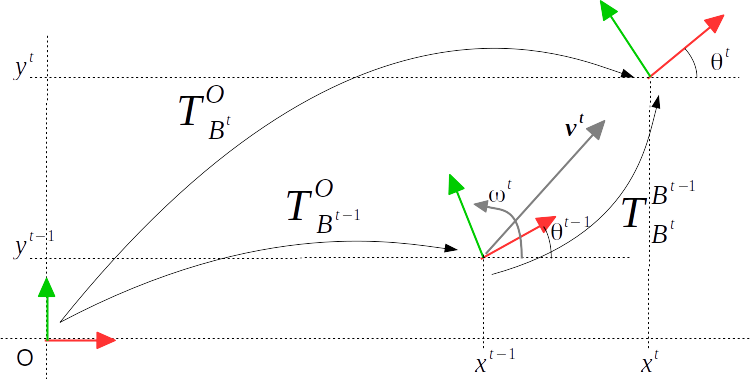
\includegraphics[width=1.0\columnwidth]{figures/odometry_integration_2d.png}
    \caption{Involved homogeneous transformations in the integration of a 2D twist. From pose at $t-1$, a twist composed of a linear velocity~$\mathbf{v}^t=[v^t_x\ v^t_y]$ and rotational velocity~$w^t_z$ is integrated to compute a pose at $t$.}
    \label{fig:odometry_integration_2d}
  \end{center}
\end{figure}

Figure~\ref{fig:odometry_integration_2d} shows the involved homogeneous transformations to compute the odometry poses. At a given discrete time $t-1$, the robot odometry pose is~$\mathbf{x^{t-1}}=[x^{t-1}\ y^{t-1}\ \theta^{t-1}]^T$, the transformation from the odometry frame up to the base (vehicle) frame is: 
\begin{equation}
 \mathbf{T}^O_{B^{t-1}} = 
 \left[
 \begin{array}{ccc}
  cos\theta^{t-1} & -sin\theta^{t-1} & x^{t-1} \\
  sin\theta^{t-1} &  cos\theta^{t-1} & y^{t-1} \\
  0 & 0 & 1
 \end{array}
 \right]
\end{equation}
At $t-1$ frame, the vehicle moves with a twist $\mathbf{u}^t=[v^t_x\ v^t_y\ w^t_z]^T$. Integrating this twist along a time increment~$\Delta\tau$, causes a pose increment expressed in vehicle frame at $t-1$, that can be represented by the following homogeneous transformation: 
\begin{equation}
 \mathbf{T}^{B^{t-1}}_{B^t} = 
 \left[
 \begin{array}{ccc}
  cos(w_z^t\Delta\tau) & -sin(w_z^t\Delta\tau) & v_x^t\Delta\tau\\
  sin(w_z^t\Delta\tau) &  cos(w_z^t\Delta\tau) & v_y^t\Delta\tau \\
  0 & 0 & 1
 \end{array}
 \right]
 \label{eq:odometry_increment}
\end{equation}
The product of the previous transformations leads to the new transformation that represents the new odometry pose at discrete time~$t$: 
\begin{equation}
\mathbf{T}^O_{B^t} = \mathbf{T}^O_{B^{t-1}} \cdot \mathbf{T}^{B^{t-1}}_{B^t}
\label{eq:odometry_transform_2D}
\end{equation}


\subsection{Uncertainty propagation in 2D}
Even if it comes from a filtering process, the twist is a noisy signal with a level of uncertainty. Therefore, the time integration explained in the previous subsection results in a pose with some degree of uncertainty too. To compute this uncertainty associated to the  odometry pose, given the twist unecrtainty, equation~\ref{eq:odometry_transform_2D} has to be linearized with respect to the twist components, prior to apply the uncertainty propagation seen at subsection~\ref{subsec:gaussian_uncertainty_propagation}: 
\begin{equation}
\mathbf{J}^{\mathbf{T}^{O}_{B^t} }_{v^t_x, v^t_y, \theta^t}= 
\mathbf{J}^{\mathbf{T}}_{\mathbf{u}} = 
 \left[
 \begin{array}{ccc}
  cos(w_z^t\Delta\tau) & -sin(w_z^t\Delta\tau) & v_x^t\Delta\tau\\
  sin(w_z^t\Delta\tau) &  cos(w_z^t\Delta\tau) & v_y^t\Delta\tau \\
  0 & 0 & 1
 \end{array}
 \right]
 \label{eq:odometry_jacobian}
\end{equation}

If the twist covariance matrix ~$\mathbf{C}^t_{\mathbf{u}}$, and the pose covariance matrix at previous iteration was~$\mathbf{C}^{t-1}_{\mathbf{x}}$, then the pose covariance at discrete time~$t$ is: 
\begin{equation}
 \mathbf{C}^t_{\mathbf{x}} = \mathbf{C}^{t-1}_{\mathbf{x}} +  
    \mathbf{J}^{\mathbf{T}}_{\mathbf{u}}
    \mathbf{C}^t_{\mathbf{u}}
    (\mathbf{J}^{\mathbf{T}}_{\mathbf{u}})^T
\end{equation}

From the above equation, it can be seen how the uncertainty associated to the odometry pose grows over time, leading to an unbounded dead reckoning pose estimation.
%\footnote{https://en.wikipedia.org/wiki/Dead_reckoning}

\subsection{Twist integration in 3D}
Given a set of vehicle 3D twists at discrete time $t$, ~$\mathbf{u}^t=[v^t_x\ v^t_y\ v^t_z\ w^t_x \ w^t_y \ w^t_z]^T$, expressed with respect to the vehicle frame at $t$, the time integration of these twists leads to a set of poses~$\mathbf{x^t}=[\mathbf{p}^t\ \mathbf{q}^t ]=[p^t_x\ p^t_y\ p^t_z\ q^t_r\ q^t_i\ q^t_j\ q^t_k]$, referenced to the initial vehicle frame. Conceptually, the integration process in 3D is the same as the process in 2D, but in terms of operations, 3D rotations allow to work in quaternion representation, so the integration equations are as follows: 
\begin{equation}
\mathbf{p}^t = \mathbf{p}^{t-1} + \mathbf{v}^t\Delta\tau
\end{equation}
for the position, and: 
\begin{equation}
\mathbf{q}^t = \mathbf{q}^{t-1}*\Delta\mathbf{q}^t
\end{equation}
for the orientation, where~$\Delta\mathbf{q}^t$ is the increment of quaternion due to rotational speed. Since~$\Delta\tau$ is usually a small time increment ($<10ms$), the rotation angle $\vert\mathbf{w}^t \vert \Delta\tau$ is usually also small, so  the increment of the quaternion can be approximated by: 
\begin{equation}
 \Delta\mathbf{q}^t \approx [1\ \frac{1}{2}w^t_x\Delta\tau\ \frac{1}{2}w^t_y\Delta\tau\ \frac{1}{2}w^t_z\Delta\tau ]^T
\end{equation}
and the orientation update can be also approximated by: 
\begin{equation}
\mathbf{q}^t = \mathbf{q}^{t-1}*\Delta\mathbf{q}^t
\approx 
\left[
 \begin{array}{cccc}
  1 & -\frac{1}{2}w^t_x\Delta\tau & -\frac{1}{2}w^t_x\Delta\tau & -\frac{1}{2}w^t_x\Delta\tau\\
  \frac{1}{2}w^t_x\Delta\tau & 1 & \frac{1}{2}w^t_x\Delta\tau & -\frac{1}{2}w^t_x\Delta\tau\\
  \frac{1}{2}w^t_x\Delta\tau & -\frac{1}{2}w^t_x\Delta\tau & 1 & \frac{1}{2}w^t_x\Delta\tau\\
  \frac{1}{2}w^t_x\Delta\tau & \frac{1}{2}w^t_x\Delta\tau & -\frac{1}{2}w^t_x\Delta\tau & 1\\
 \end{array}
 \right]
 \mathbf{q}^{t-1}
\end{equation}


\subsection{Inertial integration}
In case of using an Inertial Measurement Unit (IMU), odometry poses are computed by integrating accelerations and rotation rates read by accelerometers and gyroscopes respectively.


\subsection{Odometry sources}
There are several techniques that compute the list of poses referenced to the starting frame, called the odometry frame. They can be classified between three main approaches: (i) direct pose computation, (ii) twist time integration, (iii) inertial time integration. Table~\ref{tab:odom_sources} summarizes the main features of the most common approaches to solve the odometry problem, which is an active field in research. 
\begin{table}[hbt] \centering
\caption{Common techniques for odometry computation.}
\begin{tabular}
[c]{|c|c|c|c|c|c|c|c|}
\hline
\rowcolor{gray}    
Approach & Rate & Computational & Long-term & Short-term & Device & Typical \\
\rowcolor{gray}    
& & Complexity& drift & accuracy & mounting & application \\
\hline
Scan Matching & Low & High & Low & Medium & Delicate & Indoor \\
& & & & & & wheeled\\
\hline
Point Cloud & Low & Very High & Very Low & High & Delicate & Outdoor\\
registration & & & & & & wheeled\\
\hline
Visual & Medium & Very High & Very Low & High & Versatile & Space\\
Odometry & & & & & & Humanoids,\\
 & & & & & & Phones\\
\hline
Wheel & Medium & Low & Medium & Medium & Difficult & Wheeled\\
Encoders & & & & & & vehicles\\
\hline
Stereo & Low & Medium & Low & Medium & Rough & Automotive\\
Radar & & & & & & \\
\hline
IMU & High & Low & High & High & Versatile & Drones, \\
 & & & & & & Humanoids\\
\hline
\end{tabular}
\label{tab:odom_sources}
\end{table}

Please note that the above approaches show complementary features, therefore fusion of several approaches is highly recommended and leads to better results in both accuracy and robustness. 



%\section{Odometry}
%Odometry role, sources and 2D/3D twist integration

\newpage
\section{Map-based Localization}
particle filter localization, amcl, prediction models , likelihood models,  ...

\newpage
\input{slam.tex}

\newpage
\section{Multi-View Geometry in Computer Vision}
How points and lines change and transform from different projective views, as those taken from a camera.



\newpage
\part{Planning and Control}

\newpage
\input{planning_control.tex}


\newpage
\part{Implementation Tools and Tips}

\newpage
\section{Common Algorithms}
RANSAC, ICP, HOUGH Transform, K-means clustering

\newpage
\section{Device communication protocols}
EtherCAT, CANopen, Ethernet\/IP, SPI, SSI, 


\newpage
\bibliographystyle{plain}
\bibliography{../../../papers/bib_references/references}

\end{document}
